\documentclass[a4paper,10pt]{article}
\usepackage[utf8]{inputenc}

% ----  Useful packages % ---- 
\usepackage{amsmath}
\usepackage{graphicx}
\usepackage{amsfonts}
\usepackage{amsthm}
\usepackage{amssymb}
\usepackage{makecell}
\usepackage{tikz}
\usepackage{nccmath}
\usetikzlibrary{arrows.meta}
% ----  Useful packages % ---- 

\usepackage{wrapfig}
\usepackage{sidecap}
\usepackage{caption}
\usepackage{subcaption}
\usepackage{hyperref}
\hypersetup{
	colorlinks,
	citecolor=black,
	filecolor=black,
	linkcolor=black,
	urlcolor=black
}

% ---- Set page size and margins replace ------
\usepackage[letterpaper,top=2cm,bottom=2cm,left=3cm,right=3cm,marginparwidth=1.75cm]{geometry}
% ---- Set page size and margins replace ------

% ------- NOTA ------
\theoremstyle{remark}
\newtheorem{note}{Note}[subsection]
% ------- NOTA ------

% ------- OSSERVAZIONE ------
\theoremstyle{definition}
\newtheorem{observation}{Osservazione}[subsection]
% ------- OSSERVAZIONE ------

% ------- DEFINIZIONE ------
\theoremstyle{plain}
\newtheorem{definition}{Definizione}[subsection]
% ------- DEFINIZIONE ------

% ------- ESEMPIO ------
\theoremstyle{definition}
\newtheorem{example}{Esempio}[subsection]
% ------- ESEMPIO ------

% ------- DIMOSTRAZIONE ------
\theoremstyle{definition}
\newtheorem{demostration}{Dimotrazione}[subsection]
% ------- DIMOSTRAZIONE ------

% ------- TEOREMA ------
\theoremstyle{definition}
\newtheorem{theorem}{Teorema}[subsection]
% ------- TEOREMA ------

% ------- COROLLARIO ------
\theoremstyle{plain}
\newtheorem{corollaries}{Corollario}[theorem]
% ------- COROLLARIO ------

% ------- PROPOSIZIONE ------
\theoremstyle{plain}
\newtheorem{proposition}{Proposizione}[subsection]
% ------- PROPOSIZIONE ------

% ---- Footer and header ---- 
\usepackage{fancyhdr}
\pagestyle{fancy}
\fancyhf{}
\fancyhead[LE,RO]{A.A 2023-2024}
\fancyhead[RE,LO]{Fisica}
\fancyfoot[RE,LO]{\rightmark}
\fancyfoot[LE,RO]{\thepage}

\renewcommand{\headrulewidth}{.5pt}
\renewcommand{\footrulewidth}{.5pt}
% ---- Footer and header ---- 

% ----  Language setting ---- 
\usepackage[italian, english]{babel}
% ----  Language setting ---- 

\usepackage{listings}
\usepackage{color}

\definecolor{dkgreen}{rgb}{0,0.6,0}
\definecolor{gray}{rgb}{0.5,0.5,0.5}
\definecolor{mauve}{rgb}{0.58,0,0.82}

\lstset{frame=tb,
	language=C,
	aboveskip=3mm,
	belowskip=3mm,
	showstringspaces=false,
	columns=flexible,
	basicstyle={\small\ttfamily},
	numbers=none,
	numberstyle=\tiny\color{gray},
	keywordstyle=\color{blue},
	commentstyle=\color{dkgreen},
	stringstyle=\color{mauve},
	breaklines=true,
	breakatwhitespace=true,
	tabsize=3
}

\title{\textbf{Fisica}}
\author{Realizzato da: Matteo Giuntoni}
\date{A.A. 2023-2024}

\begin{document}
	\begin{titlepage} %crea l'enviroment
	\begin{figure}[t] %inserisce le figure
		\centering
\includegraphics[width=0.98\textwidth]{marchio_unipi_pant541.png}
	\end{figure}
	\vspace{20mm}
	
	\begin{Large}
		\begin{center}
			\textbf{Dipartimento di Informatica\\ Corso di Laurea Triennale in Informatica\\}
			\vspace{20mm}
			{\LARGE{Corso a Libera Scelta - 6 CFU}}\\
			\vspace{10mm}
			{\huge{\bf Computer Graphics}}\\
		\end{center}
	\end{Large}
	
	
	\vspace{36mm}
	%minipage divide la pagina in due sezioni settabili
	\begin{minipage}[t]{0.47\textwidth}
		{\large{\bf Professore:}\\ \large{Prof. }}
	\end{minipage}
	\hfill
	\begin{minipage}[t]{0.47\textwidth}\raggedleft
		{\large{\bf Autore:}\\ \large{Filippo Ghirardini}}
	\end{minipage}
	
	\vspace{25mm}
	
	\hrulefill
	
	\vspace{5mm}
	
	\centering{\large{\bf Anno Accademico 2023/2024 }}
	
\end{titlepage}
	
	\tableofcontents
	\newpage
	% \maketitle
	% \begin{center}
	% 	\vspace{-20pt}
	% 	\rule{11cm}{.1pt} 
	% \end{center}
	\section{Punto materiale}
Oggetto caratterizzato da una massa [kg] e da un vettore posizione [m] nello spazio 3D.
Dimensioni trascurabili, forma irrilevante rispetto ai fenomeni di interesse.
Vettore posizione come funzione del tempo t[s].
\begin{example}
    Una molecola di ossigeno se sono interessato all'aereodinamica di una vettua. 
    Un satellite attorno alla terra se ignoro le forze di marea.
\end{example}
\hspace{-15pt}\textbf{Un vettore posizione} è una funzione del tempo $t[s]$.
$$\vec{r(t)} = (x(t), y(t), z(t)) = x(t)\hat{x} + y(t)\hat{z} + z(t)\hat{z}$$
\begin{observation}
    I versori cartesiani sono costanti
\end{observation}

\begin{definition}[Legge oraria]
    Si definisce come legge oraria la funzione $t \mapsto \vec{r}(t)$.
\end{definition}

\begin{definition}[Traiettoria]
    Il luogo geometrico di punti visitati dal punto materiale.
    $$\{\vec{r}(t)\:\: per \: t \in \mathbb{R}\}$$
\end{definition}

\begin{example}
    $\vec{r}(t) = (v_0t, y_0, 0)$ e $v_0 = 3m/s, y_o = 5m$ 
    \begin{figure}[h!]
        \centering
        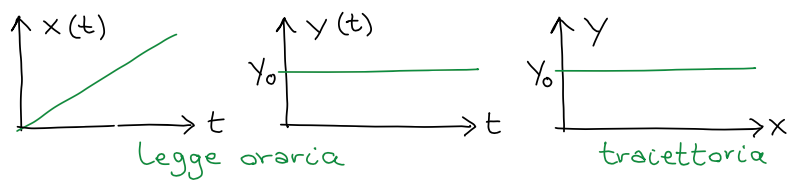
\includegraphics[width=0.8\textwidth]{images/ess-traiettoria.png}
    \end{figure}
\end{example}

\begin{definition}
    La \textbf{velocità istantanea} è la derivata della posizione rispetto al tempo.
    $$v = \lim_{\Delta t \to 0}\frac{\Delta s}{\Delta t} = \frac{ds}{dt}$$
\end{definition}

\begin{definition}
    La \textbf{velocità media} è definita come il rapporto tra lo spostamento e l'intervallo di tempo necessario per effettuarlo.
    $$v_m = \frac{\Delta s}{\Delta t}$$
\end{definition}
\hspace{-15pt}In parole povere è una grandezza che ci dice con quale rapidità cambia la posizione di un punto rispetto al tempo nell'instante $t$.
\subsection*{Vettore velocità}
Derivata rispetto al tempo del vettore posizione e si indica come 
$\frac{d\vec{r}(t)}{dt}\text{ oppure }\dot{\vec{r}}(t)[m/s]$
\begin{equation}
    \begin{split}
    \dot{\vec{r}}(t) & = (\dot{x}(t), \dot{y}(t), \dot{z}(t)) \\
     & = \frac{d}{dt}[x(t)\hat{x} + y(t)\hat{y} + z(t)\hat{z}] \\
     & = \dot{x}(t)\hat{x} + \dot{y}(t)\hat{y} + \dot{z}(t)\hat{z}
    \end{split}
\end{equation}
Per ricavare la forma esplicita uso le proprietà delle derivate (\textbf{linearità}, \textbf{Leibnitz})
\begin{example}
    $\vec{r}(t) = (v_0t, y_0, 0) = v_0t\hat{x} + y_0\hat{y}$ \:\:\:abbiamo che \:\:\:
    $\dot{\vec{r}}(t) = (v_0, 0, 0) = v_0 \hat{x}$
\end{example}
\hspace{-15pt}Velocità e spazio percorso ("integrale di linea").\\
\begin{wrapfigure}[3]{l}{5cm}
    \centering
    \includegraphics[width=5cm]{images/vettore-velocità.png}
\end{wrapfigure}
\begin{align*}
    L & = ||\vec{r}(t_1) - \vec{r}(t_0)|| + ||\vec{r}(t_2) - \vec{r}(t_1)|| + ||\vec{r}(t_3) - \vec{r}(t_2)|| + \dots \\
    & = \sum_i ||\vec{r}(t_{i+1} - \vec{r}(t_i)|| \:\: per\:\: |t_{i+1} - t_i| \text{"piccolo"} \\
    & = \sum_i ||\frac{\vec{r}(t_{i+1}) - \vec{r}(t_i)}{t_{i+1} - t_i}|| (t_{i+1} - t_i) = \int_{t_{in}}^{t_{f_{in}}}||\dot{\vec{r}}(t)||\\
\end{align*}
\begin{example}
    $\vec{r}(t) = (v_0t, y_0)\:\:\: \dot{\vec{r}}(t) = (v_0, 0)$\hspace{15pt}
    $||\dot{\vec{r}}(t)|| = \sqrt{v_0^2 + 0^2} = |v_0|$ \:\:\: $L = |v_0| \cdot (t_{f_{in}} - t_{in})$\\
    Il vettore è costante quindi facendo la derivata torna zero. Con la velocità si calcolo lo spazio percorso ("integrale di linea").
    La differenza fra le posizioni e la differenza dei tempi è il rapporto incrementale in caso gli intervalli siano sufficentemente
    piccoli, da qui si ottiene l'integrale.
\end{example}

\subsection{Vettore accelerazione}
Derivata rispetto al tempo del vettore velocità e si indica con $\frac{d^2\vec{r}(t)}{dt} \text{ oppure } \ddot{\vec{r}}(t) [m/s^2]$
\begin{equation}
    \ddot{\vec{r}}(t) = (\ddot{x}(t), \ddot{y}(t), \ddot{z}(t))\:\: = \:\: \ddot{x}(t)\hat{x} + \ddot{y}(t)\hat{y} + \ddot{z}(t)\hat{z}
\end{equation}
\begin{example}
    $\vec{r}(t)= (\frac{1}{2}a_0t^2, v_0t, 0)$ \hspace{10pt} $\dot{\vec{r}}(t) = (a_0t, v_0, 0)$ \hspace{10pt} $\dot{\vec{r}}(t) = (a_0, 0, 0)$
\end{example}
\hspace{-15pt}Serve perché l'equazione "del moto" di Newton che determinata la legge oraria è formulata in termini di accelerazione.

\subsection{Vettore quantità di moto}
Il prodotto di massa [kg] e velocità [m/s]
$$\vec{p}(t) = m \cdot \dot{\vec{r}}(t) = (m\dot{x}(t), m\dot{y}(t), m\dot{x}(t)) = m\dot{\vec{x}}(t)x + m\dot{\vec{y}}(t)y + m \dot{\vec{z}}(t)z$$
\begin{example}
    Prendiamo un punto di massa 2kg e velocità 3m/s lungo $\hat{x}$.\\
    $p_x(t) = 2 \cdot 3 kg\cdot m/s = 6 kg \cdot m/s$ \hspace{15pt} $p_y(t) = p_z(t) = 0$.
\end{example}
\hspace{-15pt}Serve per generalizzare l'equazione di Newton e per trattare sistemi di piu punti materiali.

\subsection{Vettore momento angolare rispetto a un polo P}
$$\vec{L}_p(t) = m(\vec{r}(t) - \vec{r}_p) \times \dot{\vec{r}}(t)$$
Dove $\vec{r}_p$ è il vettore posizione di p, mentre $\dot{\vec{r}}(t)$ è il prodotto vettoriale.
\begin{example}
    $\vec{r}_p = (l_0, 0, 0)$ \hspace{15pt} $\vec{r}(t) = (v_0t, y_0, 0)$\\
    $\vec{L}_p = m[(v_0t - l_0)\hat{x} + y_0\hat{y}] \times (v_0\hat{x}) \:\: = \:\: m(v_0t - l_0)v_0 \hat{x} \times \hat{x} + my_0v_0\hat{y}\times \hat{x} 
    \:\: = \:\: my_0v_0(-\hat{z}) = (0,0, -my_0v_0)$\\
    Ricorda che $\hat{x} \times \hat{x} = 0$ e $\hat{y} \times \hat{x} = -\hat{z}$
\end{example}
\hspace{-15pt}Il momento angolare dice quanta inerzia ha un oggetto in una rotazione (descrizione sommaria).\\
Il polo P è parte della definizione. È una scelta! Il risultato dipende dal polo.
Serve per formulare l'equazione del moto di sistemi di punti materiali e corpi rigidi.

\subsection{Coordinate polari}
Un metodo per rapprensentare delle cordinate x, y andando a misurare prima la distanza dall'origine e poi si va a vedere
quanto vale l'angolo fra questo segmento dall'asse x, utilizzando seno e coseno.
\begin{wrapfigure}[7]{l}{2cm}
    \centering
    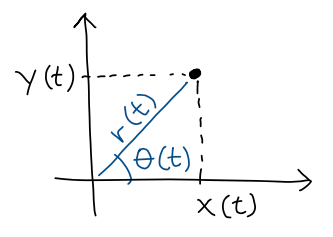
\includegraphics[width=5.5cm]{images/coordinate-polari.png}
\end{wrapfigure}
\begin{align*}
    \begin{cases}
        x(t) = r(t) \cdot \cos(\Theta(t))\\
        y(t) = r(t) \cdot \sin(\Theta(t)) 
    \end{cases}
\end{align*}
\begin{align*}
    \begin{cases}
        r(t) = \sqrt{x(t)^2 + y(t)^2} \geq 0\\
        tg(\Theta(t)) = y(t) / x(t) 
    \end{cases}
\end{align*}
\\
\begin{example} Esempi di rappresentazione di coordinate in coordinate polari.\\
    $x = 0, y = l_0 > 0 \:\: \Rightarrow \:\: r = l_0, \Theta = \pi/2$\\
    $x = 0, y = -l_0 < 0 \:\: \Rightarrow \:\: r = l_0, \Theta = -\pi/2$\\
    $x = l_0, y = l_0 > 0 \:\: \Rightarrow \:\: r = \sqrt{2}l_0, \Theta = \pi/4$\\
\end{example}

\subsection{Versori polari (2D)}
Definisco un versore $\hat{r}(t)$ che punta verso il punto materiale e un versore $\hat{\Theta}(t)$ ortogonale.
Si esprime facilmente in coordinte polari.
$$\vec{r}(t) = (x(t), y(t)) = (r(t)\cos \Theta(t), r(t)\sin\Theta(t)) \:\: = \:\: r(t)(\cos\Theta(t)\hat{x} + \sin\Theta(t)\hat{y})$$
Ma $||\vec{r}(t)|| = |r(t)| = r(t)$ allora definisco $\hat{r}(t) = \vec{r}(t)/ ||\vec{r}(t)|| = \cos \Theta(t)\hat{x} + \sin\Theta(t)\hat{y}$\\\\
Trovo facilmente che un versore ortogonale è:
$$\hat{\Theta(t)} = -\sin\Theta(t)\hat{x} + \cos\Theta(t)\hat{y} \:\:\:\text{infatti} \:\:\: \hat{r}\cdot \hat{\Theta} = c \cdot (-s) + s \cdot c = 0$$
\begin{wrapfigure}[7]{r}{6cm}
    \centering
    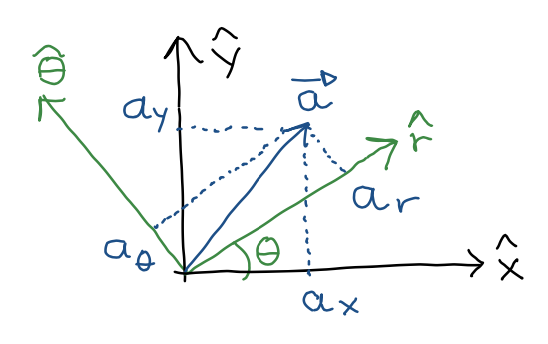
\includegraphics[width=5.5cm]{images/trasformazioni-inverse.png}
\end{wrapfigure}
\begin{note}
    Non c'è legame fra $\Theta$ e $\hat{\Theta}$ è solo una convenzione.
\end{note}
\hspace{-15pt}Le trasformazioni inverse invece si fanno come segue (verifico per sostituzione):
$$\hat{y} = \cos\Theta(t)\hat{r} - \sin\Theta(t)\hat{\Theta} \hspace{20pt} \hat{y} = \sin\Theta(t)\hat{r} + \cos\Theta(t)\hat{\Theta}$$
Possono quindi scrivere ogni vettore nella forma $\vec{a} = a_r\hat{r} + a_{\Theta}\hat{\Theta}$ con le componenti polari $a_r, a_{\Theta}$.
Per evitare ambiguità non scriviamo $(a_r, a_{\Theta})$ e riserviamo la notazione alle componenti cartesiane.\\\\
A differenza dei versori cartesiani quelli polari dipendono dal tempo per costruzioni.
$$\dot{\hat{r}}(t) = \frac{d}{dt}[\cos\Theta(t) \hat{x} + \sin\Theta(t)\hat{y}] \:\: = \:\: -\sin\Theta(t) \cdot \dot{\Theta}(t)\hat{x} + \cos\Theta(t) \cdot \dot{\Theta}(t)\hat{y}$$
Dove $\cos\Theta(t) \cdot \dot{\Theta}(t)$ si applica la derivata della somma, Leibnitz, funzione composta.
$$= \dot{\Theta}(t)\cdot \hat{\Theta}(t) \:\:\:\:(\text{confronto l'espressione di} \hat{\Theta}(t))$$
Similmente $\dot{\hat{\Theta}}(t)= - \dot{\Theta}\hat{r}(t)$.


\subsection*{Vettori posizione, velocità, accelerazione}
$$\vec{r}(t) = r(t)\hat{r}(t)$$
Dove abbiamo che $\vec{r}(t)$ è il vettore, $r(t)$ è una coordinata polare, $\hat{t}(t)$ è il versore polare.
$$\dot{\vec{r}}(r) = \dot{r}(t)\hat{r}(t) + r(t)\dot{\Theta}(t)\hat{\Theta}(t)$$
Dove la parte $\dot{\vec{r}}(r)$ è la velocità radiale.
$$\ddot{\vec{r}}(t) = [\ddot{r}(t) - r(t)\dot{\Theta}(t)^2] \hat{r} + [r(t) \ddot{\Theta}(t) + 2\dot{r}(t)\dot{\Theta}(t)]\hat{\Theta}$$
Nel quale abbiamo che la parte $r(t)\dot{\Theta}(t)^2$ si chiama \textbf{velocità centripeta}, mentre $2\dot{r}(t)\dot{\Theta}(t)$ si dice \textbf{accelerazione di Coriolis}.


	\newpage
\section{Forze}
La legge oraria $\vec{F}(t)$ di un punto materiale di massa m è determinata salla soluzione di una equzione
del moto detta \textbf{seconda legge di newton}
$$m\ddot{\vec{r}} = \vec{F}_1 + \vec{F}_2 + \dots$$
$\vec{F}_1$ sono le \textbf{forze} $[kg \cdot m/s^2 \equiv N]$ (N è l'unità di misura, Newton) agenti sul punto meteriale: sono determinate empiricamente.
L'equazione differenziale è del \textbf{secondo ordine} (derivata seconda) quindi servono due \textbf{condizioni al bordo} (si chiamano così perché indicano le 
condizioni ai bordi del dominio), ad esempio $\vec{r}(t_0) = \vec{r}_0$ e $\dot{\vec{r}}(t_0) = \vec{v}_0$ (con questa cosa stiamo dicendo che per decsrivere un moto di un sistema
dobbiamo sapere in un tempo dove il sistema si trova e la sua velocità).\\
Questa è un equazione che va a descrivere fenomeni da dimensioni incredibilmente piccole a incredibilmente grandi.\\\\
Se la somma (detta \textbf{risultate} delle forze)
$$\vec{F}_1 + \vec{F}_2 + \cdots = 0 \hspace{10pt}\text{allora}\hspace{10pt} m\ddot{\vec{r}}(t) = 0 \Rightarrow \dot{\vec{v}}(t) \equiv \vec{v}_0$$
cioè il moto ha velocità costante (\textbf{rettilineo uniforme}). Questo è in particolare vero se tutte $\vec{F}_i = 0$ 
(\textbf{prima legge di Newton} o "principio di inserzia di Galileo"). Se un corpo non è soggetto a forze esterne mantiene il suo modo rettilineo uniforme.
Questa cosa collega la proprierà di simmetria degli oggetti alla traslazione dello spazio.

\subsection{Forza costante $\vec{F} = F_0\hat{x}$}
$$\vec{r}(t) = x(t)\hat{x} + y(t)\hat{y} + z(t)\hat{z} \hspace{15pt}\ddot{\vec{r}}(t) = \ddot{x}(t)\hat{x} + \ddot{y}(t)\hat{y} + \ddot{z}(t)\hat{z}$$
$$m\ddot{\vec{r}}(t) = F_0 \hat{x} \Rightarrow 
\begin{cases}
    m\ddot{x}(t) = F_0\\
    m\ddot{y}(t) = 0\\
    m\ddot{y}(t) = 0 
\end{cases}
$$
Proietto su una base per ottenere 3 equazioni scalari. Mi servono $2 \times 3 = 6$ \textbf{condizioni al bordo} per risolvere.
Ad esempio condizioni iniziali:
$$\vec{r}(0) = \vec{r_0} = (x_0, y_0, z_0) \hspace{15pt} \dot{\vec{r}}(0) = \vec{v}_0 = (v_{0x}, v_{0y}, v_{0z})$$
$$\Rightarrow 
\begin{cases}
    x(t) = x_0 + v_{0x}t + \frac{1}{2}\frac{F_0}{m}t^2\\
    y(t) = y_0 + v_{0y}t \\
    z(t) = z_0 + v_{0z}t
\end{cases}
\Rightarrow \:\:\text{caso generale}\:\:
r(t) = r_0 + v_0t + \frac{1}{2}\frac{F_0}{m}t^2
$$
Con $t$ che rappresenta il \textbf{moto uniformamente accelerato}

\subsection{Forza peso $\vec{F} = -mg\hat{z}$}
Usata per esempio in prossimità della superficie terreste. Con $m$ massa del punto materiale dell'oggetto in cui si applica, mentre $\hat{z}$ ortogonale alla superficie. 
$g \equiv 9,8 m/s^2$, dipende da $M_T$, variazioni locali.
\begin{example}
    Grave che cade da altezza $h$.
    $$m\ddot{\vec{r}}(r) = -mg\hat{z} \hspace{15pt} \text{con}\hspace{15pt} \vec{r}(t_0) = h \cdot \hat{z}, \dot{\vec{r}}(t_0) = 0 \text{(oggetto parte da fermo)}$$
    Proietto $m\ddot{z}(t)= -mg$ \hspace{10pt} $\dot{z}(t) = -g(t - t_0)$ \hspace{10pt} $z(t) = h - \frac{1}{2}g(t - t_0)^2$\\
    Si sostituisce le costanti della soluzione per verificare che siano verificate le condizioni ai bordi.
\end{example}

\begin{example}
    Problema del proiettile.
    $$m\ddot{\vec{r}}(t) = -mg\hat{z} \:\:\text{(equazione del moto)}\:\:\: \text{con} \:\:\vec{r}(t_0) = 0$$
    $$\text{e}\:\: \dot{\vec{r}}(t_0) = v_0 \cdot \cos\Theta\hat{x} + v_0 \cdot \sin\Theta\hat{z} \hspace{10pt}\text{ovver}\hspace{10pt}\vec{v}_0 = v_0(\cos\Theta, \sin\Theta) \:\: ||\vec{v}_0|| = v_0$$
    Qui andiamo a considerare quindi una certa velocità $v_0$ con un angolo $\Theta$, e andiamo a definire la vecolità $\vec{v}_0$.
    Proiezione lungo $\hat{y}$ banale: $\ddot{y}(t) \equiv 0, y(t) \equiv 0$
    $$
    \begin{cases}
        \ddot{x}(t) = 0& \hspace{20pt} \dot{x}(t) = v_0 \cos\Theta \\
        \dot{x}(t_0) = v_0 \cos\Theta & \hspace{20pt} x(t) = v_0\cos\Theta (t-t_0)\\
    \end{cases}
    $$
    $$
    \begin{cases}
        \ddot{z}(t) = -g & \hspace{20pt} \dot{z} = v_0 \sin\Theta - g(t - t_0)\\
        \dot{z}(t_0) = v_0 \sin\Theta & \hspace{20pt} z(t) = v_0\sin\Theta(t - t_0) - \frac{1}{2}g (t - t_0)^2
    \end{cases}
    $$
    Dalla legge oraria alla traiettoria
    $$
    \begin{cases}
        x(t) = v_0 \cos\Theta(t - t_0)\\
        z(t) = v_0\sin\Theta(t - t_0) - \frac{1}{2}g(t - t_0)^2
    \end{cases}
    $$
    $$t - t_0 = x(t) \: / \: (v_0\cos\Theta) \hspace{10pt} z = v_0\sin\Theta x\: / \: (v_0 \cos\Theta) - \frac{1}{2}g x^2 \: / \: (v_0\cos\Theta)^2 \hspace{10pt} z=v_0 tg\Theta - x^2 \frac{g}{2v_0^2}\frac{1}{\cos^2\Theta}$$
    \begin{observation}
        $\frac{1}{\cos^2\Theta} = \frac{\sin^2\Theta + \cos^2\Theta}{\cos^2\Theta} = 1 + tg^2\Theta \hspace{15pt} z = x tg\Theta - x^2 \frac{g}{v_0^2}(1 + tg^2 \Theta)$ (Parabola)
    \end{observation}
    \hspace{-15pt}Punto di atterraggio: sistema con $z = 0$, $x = 0$ (banale) \hspace{10pt} $x = \frac{2v^2_0}{g}tg\Theta / (1 + tg^2 \Theta)$
\end{example}
\begin{figure}[h!]
    \centering
    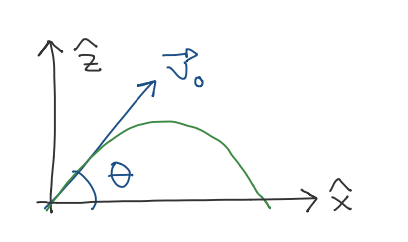
\includegraphics[width=0.3\textwidth]{images/esempio-proiettile.png}
    \caption*{Esempio proiettile}
\end{figure}

\subsection{Forza elastica $\vec{F} = -k (||\vec{r} - \vec{r}_v|| - l_0)\frac{\vec{r}-\vec{r}_v}{||\vec{r}-\vec{r}_v||}$}
\begin{wrapfigure}[7]{r}{4cm}
    \vspace{-15pt}
    \centering
    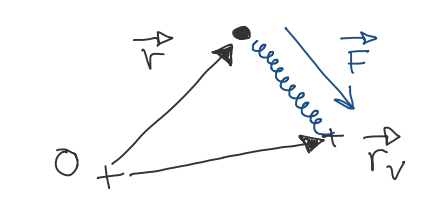
\includegraphics[width=5cm]{images/forza-elastica.png}
\end{wrapfigure}
Chiamata anche \textbf{legge di hooke}. $k$ è la costante elastica espressa in $[N/m]$ del materiale. $l_0 [m]$ lunghezza a riposo della "molla", 
dipende dal vettore posizione $\vec{r}$ ("posizionale").\\\\
$-\frac{\vec{r}-\vec{r}_v}{||\vec{r}-\vec{r}_v||}$ è il versone parallelo alla molla, cioò la distanza fra il punto di destinazione ed il vincolo, si usa perché c consente
di calcolare la forza elstica $F$ nella direzione esatta della deformazione, anziché utilizzare solo la magnitudo della deformazione ($(||\vec{r} - \vec{r}_v|| - l_0)$).
\\\\La forza elastica è tanto piu intensa quanto è estesa la molla, e questa relazione fondamentale è lineare. Una versione
più classica della legge di hooke è:
$$\vec{F} = kx$$
\begin{example}
    Oscillatore unidimensionale $\vec{r}_v = 0$.
    $$\vec{r}(t) = x(t)\vec{x}, \:\:\:x(t)\geq 0$$
    $$\vec{F}= -k(|x-0| - l_0)\frac{x - 0}{|x - 0|}\hat{x} \hspace{10pt} = \hspace{10pt} -k(|x| - l_0)\frac{x}{|x|}\hat{x} \Rightarrow F_x = -k(x-l_0)$$
    $$m\ddot{x}(t) = -k[x(t) - l_0]$$
    Soluzione generale (verifico per sostituzione)
    $$x(t) = l_0 + A \cdot \cos(\Omega t) + B \cdot \sin(\Omega t) \hspace{15pt} \Omega \equiv \sqrt{k/m}$$
    $$\dot{x}(t) = -\Omega A \sin(\Omega t) + B \Omega \cos(\Omega t)$$
    $$\Omega[rad/s] \text{la \textbf{frequenza angolare}} \hspace{10pt} \Omega/2\pi [\frac{1}{s} = Hz] \text{è la \textbf{frequenza}} \hspace{10pt} T = 2\pi/\Omega [s] \text{è il \textbf{periodo}, infatti } \Omega \cdot T = 2\pi$$ 
    Trovo $A$ e $B$ imponendo che la soluzione rispetti le condizoni al bordo, es: $x(0) = x_0, \dot{x}(0) = 0$. 
    Dalla soluzione generale ho 
    \begin{align*}
        & \dot{x}(t) = -\Omega A \sin(\Omega t) + B \Omega \cos(\Omega t) \:\: \xrightarrow{b.} \:\: 0 = -\Omega A \sin(\Omega \cdot 0) + B \Omega \cos(\Omega \cdot 0) \:\:\rightarrow\:\: 0 = 0 + B\Omega \Rightarrow B = 0\\
        & x(t) = l_0 + A \cdot \cos(\Omega t) \:\:\xrightarrow{a.}\:\: x_0 = l_0 + A \cdot \cos(\Omega \cdot 0) \:\:\rightarrow\:\: x_0 = l_0 + A
    \end{align*}
    La soluzione completa è quindi
    $$x(t) = l_0 + (x_0 - l_0) \cos(\Omega t)$$
\end{example}

\subsection{Forza di attrito viscoso $\vec{F} = -\gamma\dot{\vec{r}}(t)$}
Modello approssimato per le basse velocità. Abbiamo che $-\gamma [N/(m/s)]$ è la costante del materiale viscoso. Il meno è dato perché è una forza
che si oppone linearmente ad una velocità.
\begin{example}
    Proiettile in gel balistico.
    $$m\ddot{x}(t) = \gamma t \dot{x}(t) \:\: con \:\: \dot{x}(0) = v_0$$
    Pongo poi $u(t) \equiv \dot{x}(t) \Rightarrow \dot{u} t = -\frac{1}{\tau}u(t)$ con $u(0) = v_0$ e $\frac{1}{\tau} = \frac{\gamma}{m}[\frac{1}{s}]$\\
    Soluzione generale $u(t) = A e^{-t/\tau} \Rightarrow v_0 = A \cdot e^0 \Rightarrow v_0 = A$.\\
    Quindi la soluzione completa è
    $$u(t) = v_0 e^{-t/\tau} \:\:\: \text{ovver} \:\:\: \dot{x}(t) = v_0 e^{-t/\tau}$$
    rallentamento esponenziale.
\end{example}
\begin{figure}[h!]
    \centering
    \begin{subfigure}[b]{0.3\textwidth}
        \centering
        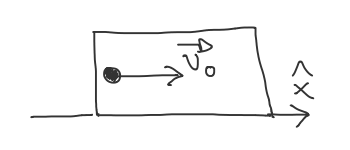
\includegraphics[width=\textwidth]{images/proiettile-gel-balistico-1.png}
        \caption*{Situazione proiettile}
    \end{subfigure}
    \begin{subfigure}[b]{0.3\textwidth}
        \centering
        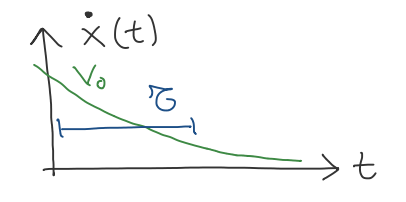
\includegraphics[width=\textwidth]{images/proiettile-gel-balitstico-2.png}
        \caption*{Soluzione completa gel}
    \end{subfigure}
\end{figure}

\subsection{Data la legge oraria, trovare la forza}
$r(t) = R, \Theta(t) = \Omega t$ \textbf{moto circolare uniforme}
$$\vec{r}(t) = r(t)\hat{r}\hspace{15pt}\hat{r} = \cos(\Theta(t))\hat{x} + \sin(\Theta(t))\hat{t}$$
$$\ddot{\vec{r}} (t) = [\ddot{r(t)} - r(t)\dot{\Theta}(t)^2]\hat{r} + [r(t)\ddot{\Theta}(t) + 2\dot{r}\dot{\Theta}(t)]\hat{\Theta}$$
Dalla legge oraria ho: $\dot{x}(t) = 0, \ddot{r}(t) = 0, \dot{\Theta} = \Omega, \ddot{\Theta}(t) = 0 \Rightarrow$ in questo caso $\ddot{\vec{r}}(t) = -R\Omega^2\hat{r}$.\\
La risultate $\vec{F}$ delle forze deve essere tale che $m\ddot{\vec{r}}(t) = \vec{F} \Rightarrow -mR\Omega^2\hat{r} = \vec{F} \Rightarrow \vec{F} = -mR\Omega\vec{r}$.\\
La forza è costante e sempre diretta verso lo stesso punto (\textbf{forza centrale} o  \textbf{forza centripeda}). Ottengo $\vec{F}$ solo per questa legge oraria.\\\\
Integrazione numeria delle equazioni del moto.

\subsection{Discretizzare la varibile temporale}
Calcolo al "primo ordine" ("metodo di eulero"), ci sono anche molti altri agloritmi come per esempio Runge-Kutta, la scelta
dipende dal problema.
$$t \to t_0, t_1, \dots, t_n \hspace{15pt} t_{i+1} - t_i = \Delta t \hspace{15pt}\vec{r}(t_i) = \vec{r}_i$$
$$\frac{d\vec{r}(t)}{dt}|_{t=t_i} \simeq \frac{\vec{r}_{i+1} - \vec{r}_i}{\Delta t} \hspace{20pt}\frac{d^2\vec{r}(t)}{dt}|_{t = t_i} \simeq \frac{\frac{\vec{r}_{i+1} - \vec{r}_i}{\delta t} - \frac{\vec{r}_i - \vec{r}_{i-1}}{\Delta t}}{\Delta t} = \frac{\vec{r}_{i+1} - 2 \vec{r}_i - \vec{r}_{i-1}}{\Delta t^2}$$
L'equazione di Newton diventa:
$$\vec{v}_i = \vec{v}_{i-1} + \Delta t \vec{F}_{i-1} / n \hspace{20pt}\vec{r}_i = \vec{r}_{i-1} + \Delta t \vec{v}_i$$
Servono 2 condizioni al bordo $\vec{F}_i$ può dipendere da $t_i, \vec{r}_i, \vec{v}_i$

\newpage
\section{Reazioni vincolari}
Estendiamo il modello del "punto materiale" all'interazione di corpi estesi in moto tralatorio
$\Delta \vec{r}_i = \Delta \vec{r}_2$ per ogni punto posso studiare una qualsiasi $\vec{r}(t)$
\begin{itemize}
    \item La \textbf{traslazione} può avvenire su una traiettoria curva, parleremo di \textbf{rotazione} più avanti.
    \item Consideriamo il \textbf{contatto} tra punti materiali, corpi estesi, superfici.
\end{itemize}
Le forze di contatto ("reazioni vincolari") non sempre hanno una espressione esplicita e vengono determinate imponendo dei vincoli alle 
equazioni del moto, ad esempio che un punto segua una data traiettora.
\begin{figure}[h!]
    \vspace{-10pt}
    \centering
    \begin{subfigure}[b]{0.25\textwidth}
        \centering
        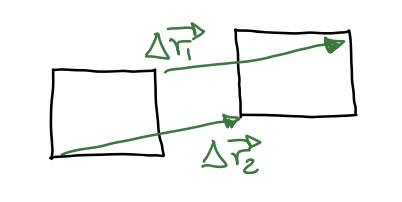
\includegraphics[width=\textwidth]{images/reazioni-vincolari-intro-1.png}
        \caption*{Traslazione punto materilae}
    \end{subfigure}
    \begin{subfigure}[b]{0.25\textwidth}
        \centering
        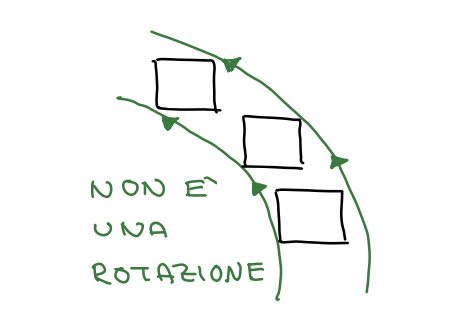
\includegraphics[width=\textwidth]{images/reazioni-vincolari-intro-2.png}
        \caption*{Rettilineo curvo}
    \end{subfigure}
    \begin{subfigure}[b]{0.4\textwidth}
        \centering
        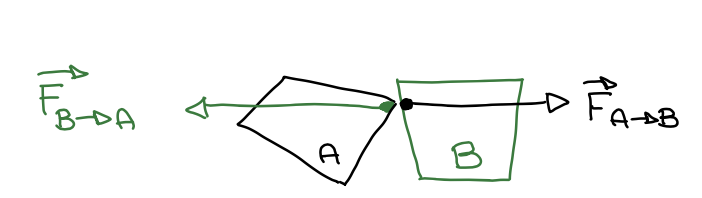
\includegraphics[width=\textwidth]{images/reazioni-vincolari-intro-3.png}
        \caption*{Contatto fra corpi}
    \end{subfigure}
\end{figure}
\begin{example} \label{es-rez-vin-1}
    $x(t) \equiv x_0$ 
\end{example}
\hspace{-15pt}La "terza legge di Newton" ("azione e reazione") stabilisce che $\vec{F}_{B\to A} = -\vec{G}_{A \to B}$
\begin{example} \label{es-rez-vin-2}
    Massa su una bilancia in presenza di forza peso.
    $$m\ddot{\vec{r}}(t) = -mg\hat{z} + \vec{F}$$
    In questo caso il \textbf{Vincolo} è: 
    $$\dot{\vec{r}}(t) = 0 \:\:\:\Rightarrow\:\:\: \vec{F} = +mg\hat{z}$$ 
    La bilancia misura $||-\vec{F}|| = mg$ (che noi chiamiamo comunemente peso).
\end{example}
\begin{example} \label{es-rez-vin-3}
    Massa su bilancia in ascesore accelerato.
    $$m\ddot{\vec{r}}(t) = -mg\hat{z} + \vec{F}$$
    Ciò che cambia ora è il suo \textbf{Vincolo} visto che si sta accelerando vesto l'alto: 
    $$\ddot{\vec{r}}(t) \equiv a \cdot \hat{z} \:\:\:\Rightarrow\:\:\: \vec{F}= m(a+g)\hat{z}$$
    La bilancia misura $||-\vec{F}|| = m(a+g)$.
    La bilancia allora misura una forza peso maggiore in un ascensore (stiamo usando l'equazione "al contrario").
\end{example}
\begin{note}
    Un punto materiale si "solleva", si "distacca" da una superfice quando la reazione vincolare va a zero.
\end{note}
\begin{figure}[h!]
    \vspace{-10pt}
    \centering
    \begin{subfigure}[b]{0.25\textwidth}
        \centering
        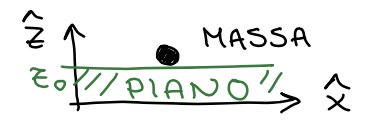
\includegraphics[width=\textwidth]{images/esempio-reazioni-vincolari-1.png}
        \caption*{Esempio \ref{es-rez-vin-1}}
    \end{subfigure}
    \begin{subfigure}[b]{0.25\textwidth}
        \centering
        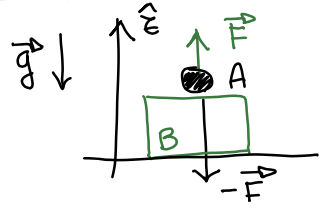
\includegraphics[width=\textwidth]{images/esempio-reazioni-vincolari-2.png}
        \caption*{Esempio \ref{es-rez-vin-2}}
    \end{subfigure}
    \begin{subfigure}[b]{0.2\textwidth}
        \centering
        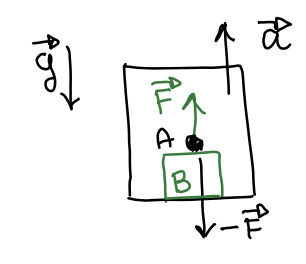
\includegraphics[width=\textwidth]{images/esempio-reazioni-vincolari-3.png}
        \caption*{Esempio \ref{es-rez-vin-3}}
    \end{subfigure}
\end{figure}
\hspace{-15pt}Scomponiamo la reazione vincolare nella direzione
\begin{itemize}
    \item ortogonale: "reazione normale" $\vec{N}$".
    \item parallelo: "forza di \textbf{attrito}" $\vec{F}_a$
\end{itemize}
\newpage
\begin{wrapfigure}[6]{r}{4cm}
    \centering
    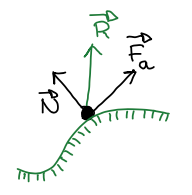
\includegraphics[width=2.7cm]{images/scomposizione-reazione-vincolare.png}
\end{wrapfigure}
ad una superficie. Con una superficie \textbf{liscia} abbiamo $\vec{F}_a = 0$, non c'è
movimento relativo al punto di contatto.
\textbf{Attrito statico}, $\vec{F}_a$ da determinare con vincoli. Condizione: $$||\vec{F}_a|| \leq \mu_s ||\vec{N}||$$
Differenza di velocità $\vec{v}$ al punto di contatto. \textbf{Attrito dinamico}:
$$\vec{F}_a = -\mu_a ||\vec{N}||\frac{\vec{v}}{||\vec{v}||}$$
$\mu_s, \mu_d$: coeff. di attrito, numeri primi.
$-\frac{\vec{v}}{||\vec{v}||}$ diretto in versione opposta alla velocità.

\begin{example}\label{es-rez-vin-4}
    Massa su un piano inclinato liscio e fisso.
    $$\hat{x}' = \cos\alpha \cdot \hat{x} - \sin\alpha \cdot \hat{z} \hspace{20pt}\hat{z}' = \sin\alpha \cdot \hat{x} + \cos\alpha \cdot \hat{z} \hspace{15pt} m\ddot{\vec{r}}(t) = -mg\hat{z} + \vec{N}$$
    \begin{itemize}
        \item Proietto lungo $\hat{z}'$: \hspace{15pt} $m\ddot{z}'(t) = -mg\cos\alpha + N$
        \item Proietto lungo $\hat{x}'$: \hspace{15pt} $m\ddot{x}'(t) = +mg\sin\alpha$.
    \end{itemize}
    Vincolo: $z'(t) = \cos t \hspace{10pt} \ddot{z}'(t) = 0\:\:\: \Rightarrow\:\:\: N = mg\cos\alpha \hspace{20pt} \ddot{x}'(t) = g \cdot \sin\alpha$\\
    Visto che $\sin\alpha < 1$ quindi l'accelerazione lungo il piano è $< g$.
\end{example}

\begin{example}\label{es-rez-vin-5}
    Massa ferma su piano inclinato scabro.
    $$m\ddot{z}'(t) = -mg\cos\alpha + N \hspace{20pt} m\ddot{x}'(t) = +mg\sin\alpha - F_{a}$$
    La scelta fra $-F_{a}$ o $+F_a$ è indifferente, l'unica cosa che cambia è nel risultato poi sarà diverso il segno di $F_a$, la coorenza da tenere è riguardante il disegno, se si disegna
    in una determinata direzione, si cerca di mettere il segno uguale.
    \begin{itemize}
        \item Vincolo: $z'(t) = \cos t \:\:\:\Rightarrow\:\:\: \ddot{z}'(t) = 0 \:\:\:\Rightarrow\:\:\: N = mg\cos\alpha$.
        \item Vincolo: $x'(t) = \cos t \:\:\:\Rightarrow\:\:\: \ddot{x}'(t) = 0 \:\:\:\Rightarrow\:\:\: F_a = mg\sin\alpha$
    \end{itemize}
    Qual'è il massimo valore di $\alpha$?
    $$||\vec{F}_a|| \leq \mu_s ||\vec{N}|| \:\:\:\Rightarrow\:\:\: mg\sin\alpha \leq \mu_s \cdot mg \cos\alpha \hspace{15pt} \tan\alpha \leq \mu_s \hspace{10pt} \alpha \leq \arctan\mu_s$$
\end{example}

\begin{example}\label{es-rez-vin-6}
    Massa scivola su piano inclinato scabro.
    $$m\ddot{z}'(t) = -mg\cos\alpha + N \hspace{20pt} m\ddot{x}'(t) = +mg\sin\alpha - F_{a}$$
    Vincolo: $z'(t) = \cos t \:\:\:\Rightarrow\:\:\: \ddot{z}'(t) = 0 \:\:\:\Rightarrow\:\:\: N = mg\cos\alpha$\\
    Forza di attrito dinamico: 
    $$F_a = \mu_{\alpha}N \:\:\:\Rightarrow\:\:\: m\ddot{x}'(t) = mg\sin\alpha - \mu_{\alpha} \cdot mg\cos\alpha \hspace{15pt} \ddot{x}'(t) = g(\sin g - \mu_{\alpha} \cdot \cos \alpha)$$
    Accelerazione costante, minore che senza attrito.
\end{example}

\begin{figure}[h!]
    \vspace{-10pt}
    \centering
    \begin{subfigure}[b]{0.25\textwidth}
        \centering
        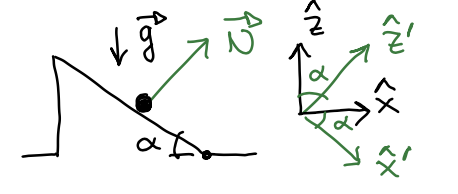
\includegraphics[width=\textwidth]{images/esempio-reazioni-vincolari-4.png}
        \caption*{Esempio \ref{es-rez-vin-4}}
    \end{subfigure}
    \hspace{20pt}
    \begin{subfigure}[b]{0.25\textwidth}
        \centering
        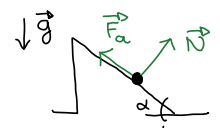
\includegraphics[width=\textwidth]{images/esempio-reazioni-vincolari-5.png}
        \caption*{Esempio \ref{es-rez-vin-5}}
    \end{subfigure}
    \hspace{20pt}
    \begin{subfigure}[b]{0.2\textwidth}
        \centering
        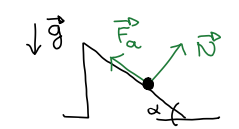
\includegraphics[width=\textwidth]{images/esempio-reazioni-vincolari-6.png}
        \caption*{Esempio \ref{es-rez-vin-6}}
    \end{subfigure}
\end{figure}
	\newpage
\section{Energia}
\subsection{Energia cinetica}
Definiamo \textbf{energia cinetica} di un punto materiale come:
$$k(t) = \frac{1}{2}m||\dot{\vec{r}}(t)||^2 \hspace{15pt} [k] = kg \cdot m^2/s^2 \equiv J \text{"Joule"}$$
La parte di $\frac{1}{2}$ sta per convenzione/comodità, le prime definizioni nel 900 infatti non lo aveva.
\begin{example}
    $\vec{r}(t) = v_0 \cap{x} \hspace{15pt} k= \frac{1}{2}mv_0^2$
\end{example}
Definiamo \textbf{lavoro} di una forza $\vec{F}(t)$ applicata nella posizione $\vec{r}(t)$ per $t_0 \leq t \leq t_1$
$$L(t_0, t_1) = \int_{t_0}^{t_1}dt \vec{F}(t) \cdot \dot{\vec{r}}(t) \hspace{15pt} [L] = s \cdot N \cdot \frac{m}{s} = J$$
\begin{example}
    $\vec{r} = v_0 \hat{x} \hspace{15pt} \vec{F}(t) = \alpha t \hat{x} + \beta \hat{y} \hspace{15pt} L(t_0, t_1) = \int_{t_0}^{t_1} dt(\alpha t\hat{x} + \beta \hat{y}) \cdot v_0 \hat{x} = \alpha v_0 \frac{t_1^2 - t_0^2}{2}$
\end{example}

\begin{theorem}[Delle forze vive]
    Per un punto materiale, la variazione di energia cinetica è pari al lavoro delle forze.
    $$K(t_1) - K(t_0) = L_1(t_0, t_1) + L_2(t_0, t_1) + \dots$$
\end{theorem}
\hspace{-15pt}Segue dalla seconda legge di Newton:
\begin{equation*}
    \begin{split}
        \sum_{i} d\alpha_i(t) & = \sum_i dt \cdot \vec{F}(t) \cdot \dot{\vec{r}}(t) = dt (\sum_i \vec{F_1}(t)) \cdot \dot{\vec{r}}(t)\\
                              & = dt \cdot m \ddot{\vec{r}}(t) \cdot \dot{\vec{r}}(t) = dt \cdot m \cdot \frac{1}{2}\frac{d}{dt}||\dot{\vec{r}}(t)||^2\\
                              & = \frac{1}{2}md||\dot{\vec{r}}(t||^2 \:\: \text{e integro membro a membro.}
    \end{split}
\end{equation*}
Se la forza dipende solo dalla posizione di applicazione $\vec{r}(t)$, ma non esplicitamente dal tempo t, si dice \textbf{posizionale}. Questo vuol
dire che, se immaginiamo un punto materiale che fa un determianta legge oraria, man mano che il punto materiale si muove il suo valore cambia, ed anche la forza 
cambia, quindi cambia in base alla posizione.
\begin{example}
    $\vec{F}(\vec{r}(t)) = \vec{F}(x(t), y(t)) = \alpha x(t) \hat{x} + \beta y(t) \hat{y}$
\end{example}
\hspace{-15pt}La dipendenza dal tempo è determinata dall'eventuale movimento della posizione di applicazione. È ben definita $\vec{F}(\vec{r}) \forall t$. \\\\
Per una forza posizione il lavoro si semplifica e diventa:
\begin{equation*}
    \begin{split}
        L(t_0, t_1) & = \int_{t_0}^{t_1}dt \vec{F}(t) \cdot \dot{\vec{r}}(t) = \int_{t_0}^{t_1}dt \vec{F}(\vec{r}(t)) \cdot \dot{\vec{r}}(t) \\
                    & = \sum_i \Delta t_i \vec{F}(\vec{r_i}) \cdot \frac{\vec{r_{i+1}} - \vec{r_i}}{\Delta t_i} = \int_{\vec{r}(t_0 )}^{\vec{r}(t_i)} d\vec{r}\cdot \vec{F}(\vec{r}) = L_e \:\:\text{"integrale di lena"}
    \end{split}
\end{equation*}
Dipende dalla traiettoria, non dalla legge oraria.
\begin{example}
    $\vec{F}(x)= -kx\hat{x} \hspace{20pt} \vec{r}(t) = v_0 \cdot \cos(\Omega t)\hat{x}$\\
    $t_0 = 0, \vec{r}(t_0) = x_0 \hat{x}, \hspace{15pt} t_1 = \frac{\pi}{\Omega}, \hspace{15pt} \vec{r}(t_1) = x_0 \cdot (-1)\hat{x}$\\
    $L(t_0, t_1) = \int_{x_0}^{-x_0}dx \hat{x} \cdot (-kx\hat{x}) = -k \frac{x^2}{2} |_{x_0}^{-x_0} = -k x_0^2 \:\: \text{non dipende da }\Omega$
\end{example}
% DA CORREGGERE seguendo nuovo pdf
\begin{observation}
    Per calcolare l'integrale di linea può comunque convenire la formula $\int_{t_0}^{t_1}dt \vec{F}(\vec{r}(t))$. 
    $\dot{\vec{r}}(t)$ eventualmente usando una legge oraria più semplice con medesima traiettoria.
\end{observation}
\begin{example}
    $\vec{F}(\vec{r}) = -kx\hat{x} \hspace{15pt}\vec{r}(t) = R\vec{r}, \Theta(t) = \Omega t \Rightarrow x(t) = R \cos(\Omega t)$\\
    $t_0 = 0, \Theta(t_0) = 0, \hspace{10pt}t_1 = \frac{\pi}{2\Omega}, \Theta(t_1) = \frac{\pi}{2} \hspace{10pt} \dots d\vec{r}\dots \hspace{15pt} \dot{\vec{r}}(t) = R\Omega\hat{\Theta} = -R\Omega\sin(\Omega t)\hat{x} + R\Omega \cos(\Omega t)\hat{y}$
    \begin{equation*}
        \begin{split}
            L(t_0, t_1) & = \int_{t_0}^{t_1}dt \vec{F}(\vec{r}(t)) \cdot \dot{\vec{r}}(t) = \int_{0}^{\pi/2\Omega}[-k R \cos(\Omega t)\hat{x}] \cdot [-R \Omega \sin(\Omega t) \hat{x} + R\Omega \cos(\Omega t)\hat{y}]\\
                        & = \int_{0}^{\pi/2\Omega}kR^2 \Omega \frac{1}{2}\sin(2\Omega t \:\: (\equiv \alpha) \:\:) = kR^2 \Omega \frac{1}{2}\int_{0}^{\pi} \frac{d\alpha}{2\Omega}\sin\alpha = \frac{1}{4} kR^2[-\cos\alpha] = \frac{1}{2}kR^2 
        \end{split}
    \end{equation*}
\end{example}
\hspace{-15pt}Se la forza è \textbf{uniforme} lungo il percorso abbiamo
$$L(t_0, t_1) = \vec{F} \cdot \int_{\vec{r}(t_0)}^{\vec{r}(t_1)} = \vec{F} \cdot [\vec{r}(t_1) - \vec{r}(t_0)] \:\text{(spostamento)}$$
\begin{example}
    $\vec{F}(\vec{r}) = \vec{F}(z) = -mg\hat{z}$ (uniforme ovunque).\\
    $\vec{r}(t) = v_0 t\hat{z} \hspace{20pt} t_0 = 0 \vec{r}(t_0) = 0 \hspace{20pt} t_1 = \frac{h}{v_0} \vec{r}(t_1) = h\hat{z} \hspace{20pt}L(t_0, t_1) = \int_{0}^{hat}dz \hat{z} \cdot (-mg\hat{z}) = -mgh$
\end{example}
\hspace{15pt}Una forza posizione si dice \textbf{conservativa} e il lavoro non dipende dal percorso, ma solo dalle posizioni iniziali e finali.
Questo accade se e solo se esiste una funzione $u(\vec{r})$ detta \textbf{potenziale} tale che:
$$\vec{F}(\vec{r}) = -\vec{\nabla}u(\vec{r}) \equiv (-\frac{d}{dx}u(\vec{r}), -\frac{d}{dy}u(\vec{r}), -\frac{d}{dz}u(\vec{r}))$$
In tal caso $\int_{\vec{r_0}}^{\vec{r_1}} d\vec{r} \cdot \vec{F}(\vec{r}) = u(\vec{r}_0) - u(\vec{r}_1)$
\begin{itemize}
    \item Forza peso: $u(\vec{r}) = mgz \hspace{20pt} \frac{d}{dx}u(\vec{r}) = \frac{d}{dy}u(\vec{r}) = 0 \hspace{10pt} \frac{d}{dz}u(\vec{r}) = mg \Rightarrow \vec{\nabla}u(\vec{r}) = (0,0, mg)= mg\hat{z} \Rightarrow \vec{F}= -kx\hat{z}$
    \item Oscillatore unidimensionale: $u(\vec{r}) = \frac{1}{2}kx^2 \hspace{20pt} \frac{d}{dy}u(\vec{r}) = \frac{d}{dz} u(\vec{r}) = 0 \hspace{10pt} \frac{d}{dx}u(\vec{r}) = kx \Rightarrow \vec{\nabla}u(\vec{r}) = (kx, 0, 0) = kx\hat{x} \Rightarrow \vec{F} = -kx\hat{x}$
\end{itemize}
\begin{observation}
    Una forza non posizionale (es. reazioni vincolari) non può essere conservativa.
\end{observation}

\subsection{Energia meccanica}
\hspace{-15pt}Il potenziale è definito "a meno di una costante" perché $-\vec{\nabla}[u(\vec{r}) + u_0] = -\vec{\nabla}u(\vec{r})$. Es: $mg(z-z_0)$
Per un punto materiale, la somma di energia cinetica e dei potenziali delle forze (conservative) alle quali è soggetto (calcolati nella sua posizione) si 
dice \textbf{energia meccanica}.
$$E(t) = K(t) + u_1(\vec{r}(t)) + u_2(\vec{r}(t)) + \cdots$$
Dal teorema delle forze vive segue che la variazione di energia meccanica è pari al lavoro delle forze \textbf{non conservatie}
$$E(t_1) - E(t_0) = L_1^{NC}(t_0, t_1) + L_2^{NC}(t_0, t_1) + \cdots$$
Se $L_i^{NC} = 0$ l'energia meccanica è \textbf{costante} nel tempo ("conservata").\\\\
Il profilo del potenziale visualizza le forze.
% Inserisci le immagine 
\begin{figure}[h!]
    \centering
    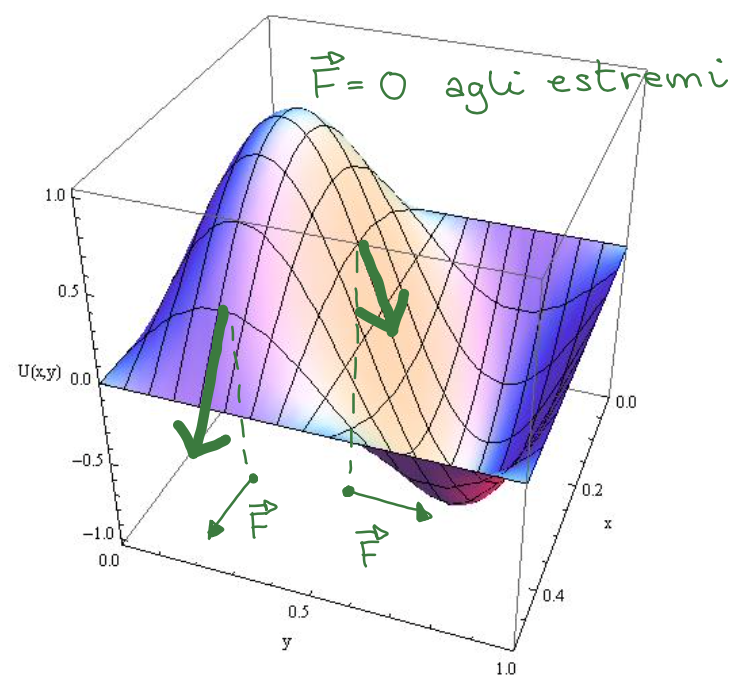
\includegraphics[width=0.28\textwidth]{images/profilo-potenziale.png}
\end{figure}
\newpage
Il profilo di potenziale visualizza le regioni dove il moto è permesso se l'energia è conservata.
\begin{figure}[h!]
    \centering
    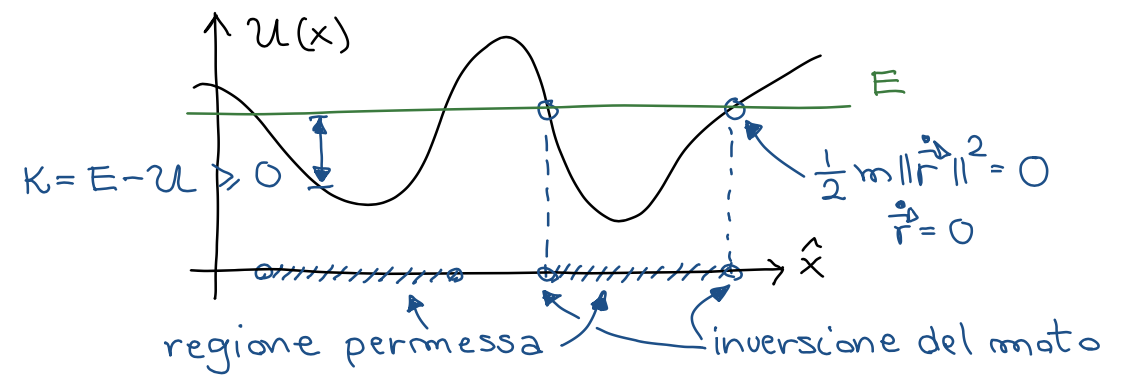
\includegraphics[width=0.75\textwidth]{images/regioni-permesse-profilo-potenziale.png}
\end{figure}
\begin{observation}
    Il "tunneling" tra regioni permesse disgiunte è possibile per atomi e particelli subatomiche secondo
    le leggi della \textbf{meccanica quantistica}.
\end{observation}

	\newpage
\section{Sistemi di punti matariali}
Consideriamo un insieme ("sistema") di punti materiali. Deduciamo delle equazioni del moto e leggi di conservazione 
come conseguenza delle leggi di Newton.
\begin{itemize}
    \item Sistemi di punti molto molto numerosi possono dare origine a fenomeni emergenti (es. sistemi biologici) \textbf{"More is different"}
    \item Concetti utili sono introdotti da teorie non riduzionistiche.
\end{itemize}
Punti $\{\vec{r}_{\alpha}\}^N_{\alpha=1}$ con masse $\{m_{\alpha}\}^N_{\alpha = 1}$ etc. Risultate delle forze su ogni punto $\{\vec{F}_{\alpha}\}^N_{\alpha = 1}$.
Quantità definite per il sistema:
\begin{itemize}
    \item \textbf{Massa} $$M = \sum_{\alpha = 1}^{N}m_{\alpha}$$
    \item \textbf{Vettore quantià di moto} $$\vec{P}(t) = \sum_{\alpha = 1}^{N} \vec{P}_{\alpha}(t)$$
    \item \textbf{Vettore momento angolare rispetto ad un polo P} $$\vec{L}_p(t) = \sum_{\alpha = 1}^{N}\vec{L}_{p, \alpha}(t) \:\:\: \text{stesso P per ogni }\alpha$$
    \item \textbf{Energia cinetica} $k(t) = \sum_{\alpha=1}^{N}k_{\alpha}(t)$
    \item \textbf{Energia meccanica} $E(t) = \sum_{\alpha=1}^{N}E_{\alpha}(t)$
\end{itemize}
Nel caso di sistemi estrmamente numerosi (es. atomi di gas, elettroni in un metallo, granelli di sabbia in una duna), può convenire
considerare il sistema \textbf{continuo}.
\begin{itemize}
    \item $n(\vec{r})$: numero di punti in un volumetto $V$ attorno a $\vec{r}$, diviso per $V$ $[n] = m^{-3}$
    \item $g(\vec{r})$: massa in un volumetto V attorno a $\vec{r}$ diviso per V (\textbf{"densità"}) $[g] = kg \cdot m^{-3}$
\end{itemize}
\begin{observation}
    Il risultato non deve dipendere dal valore preciso di V, ma l'ordine di grandezza dipende dal problema (es. densità della terra...?)
\end{observation}
\begin{definition}
    Definisco \textbf{centro di massa} del sistema di punti di materiali il punto geometrico 
    $$\vec{r}_{CM} = \frac{1}{M}\sum_{\alpha = 1}^{N} m_{\alpha}\vec{r}_{\alpha}(t)$$
\end{definition}
\begin{example}
    $\vec{r}_1(t) = v_0 t \hat{x} + y_0 \hat{y} \:\:\: m_1 = m \hspace{10pt} \vec{r}_2(t) = -2v_0 t \hat{x} + 2y_0 \hat{y} \:\:\: m_2 = 3m$
    $$\vec{r}_{CM} = \frac{1}{m + 3m}[(mv_0t - 6mv_0t)\hat{x} + (my_0 + 6my_0)\hat{y}] = \frac{1}{4m}[-5mv_0t\hat{x} + 7my_0 \hat{y}] = -\frac{5}{4} v_0t\hat{x} + \frac{7}{4}y_0\hat{y}$$
\end{example}
\begin{observation}
    Il CM non è un punto fisico, può trovare fuori dalla regione spaziale occupata dal sistema.
\end{observation}
Posso indicare ogni punto materiale con la posizione relativa al CM:
$$\vec{r}_{\alpha}'(t) = \vec{r}_{\alpha} - \vec{r}_{CM}(t)$$
Osservo che 
$$\sum_{N}^{\alpha = 1}m_{\alpha}\vec{r}'_{\alpha}(t) = \sum_{\alpha = 1}^{N}[n_{\alpha}\vec{r}_{\alpha}(t) - m_{\alpha}\vec{r}_{CM}(t)] = M\vec{r}_{CM}(t) - (\sum_{\alpha = 1}^{N}m_{\alpha})\vec{r}_{CM}(t) = 0$$
Esprimo il vettore quantità di moto:
$$\vec{p}(t) = \sum_{\alpha = 1}^{N}\dot{\vec{r}}_{\alpha}(t) = \sum_{\alpha = 1}^{N}m_{\alpha}[\dot{\vec{r}}_{CM} + \dot{\vec{r}}'_{\alpha}(t)]
= \Big(\sum_{\alpha = 1}^{N}m_{\alpha}\Big)\dot{\vec{r}}_{CM}(t) = \frac{d}{dt} \Big(\sum_{\alpha=1}^{N}m_{\alpha}\vec{r}_{\alpha}'(t)\Big) = M\dot{\vec{r}}_{CM}(t)
$$ 
ma non è un punto materiale. \\
Esprimo il vettore momento angolare rispetto a P:
\begin{equation*}
    \begin{split}
        \vec{L}_p(t) & = \sum_{\alpha=1}^{N}m_{\alpha}(\vec{r}_{\alpha} - \vec{r}_p(t)) \times \dot{\vec{r}}_{\alpha}(t) = \sum_{\alpha=1}^{N} m_{\alpha}(\vec{r}_{CM}(t) + \vec{r}'_{\alpha}(t) - \vec{r}_p(t)) \times (\dot{\vec{r}}_{CM} + \dot{\vec{r}}_{\alpha}'(t))\\
                     & = \sum_{\alpha=1}^{N}m_{\alpha}\big\{(\vec{r}_{CM}(t) - \vec{r}_p(t))\times \dot{\vec{r}}_{CM}(t) + \vec{r}_{\alpha}'\times \dot{\vec{r}}_{\alpha}'(t) + (\vec{r}_{CM}(t) - \vec{r}_p(t)) \times \dot{\vec{r}}_{\alpha}'(t) + \vec{r}_{\alpha}'(t) \times \dot{\vec{r}}_{CM}(t) \big\}\\
                     & = \bigg(\sum_{\alpha=1}^{N}m_{\alpha}(\vec{r}_{CM}(t) - \vec{r}_p(t)) \times \dot{\vec{r}}_{CM}(t) + \sum_{\alpha=1}^{N}m_{\alpha}\vec{r}_{\alpha}' \times \dot{\vec{r}}_{\alpha}'(t)\bigg) + (\vec{r}_{CM}(t) - \vec{r}_p(t)) \times \frac{d}{dt}(\sum_{\alpha=1}^{N} m_{\alpha} \vec{r}_{\alpha}'(t))\\
                     & + (\sum_{\alpha=1}^{N} m_{\alpha}\vec{r}_{\alpha}'(t)) \times \dot{\vec{r}}_{CM}(t) = M(\vec{r}_{CM}(t) - \vec{r}_p(t)) \times \dot{\vec{r}}_{CM}(t) + \sum_{\alpha=1}^{N}m_{\alpha}\vec{r}_{\alpha}'(t) \times \dot{\vec{r}}_{\alpha}'(t)
    \end{split}
\end{equation*}
$M(\vec{r}_{CM}(t) - \vec{r}_p(t)) \times \dot{\vec{r}}_{CM}(t)$ del CM. $\sum_{\alpha=1}^{N}m_{\alpha}\vec{r}_{\alpha}'(t) \times \dot{\vec{r}}_{\alpha}'(t)$ rispetto al CM. Ma non è un punto materiale.\\
Esprimo l'energia cinetica:
\begin{equation*}
    \begin{split}
        K & = \sum_{\alpha=1}^{N}\frac{1}{2}m_{\alpha}||\dot{\vec{r}}_{\alpha}(t)||^2 = \sum_{\alpha=1}^{N}\frac{1}{2}m_{\alpha}(\dot{\vec{r}}_{CM}(t) + \dot{\vec{r}}_{\alpha}'(t)) \cdot (\dot{\vec{r}}_{CM}(t) + \dot{\vec{r}}_{\alpha}'(t))\\
          & = \sum_{\alpha=1}^{N}\frac{1}{2}m_{\alpha}[||\dot{\vec{r}}_{CM}(t)||^2 + ||\dot{\vec{r}}_{\alpha}'(t)|| + 2\dot{\vec{r}}_{\alpha}'(t) \cdot \dot{\vec{r}}_{CM}(t)] = \frac{1}{2}(\sum_{\alpha=1}^{N}m_{\alpha}) ||\dot{\vec{r}}_{CM}||^2 \\
          & + \sum_{\alpha=1}^{N}\frac{1}{2}m_{\alpha}||\dot{\vec{r}}_{\alpha}(t)||^2 + 2(\sum_{\alpha=1}^{N}m_{\alpha}\dot{\vec{r}}_{\alpha}'(t)) \cdot \dot{\vec{r}}_{CM}(t) = \frac{1}{2}M ||\dot{\vec{r}}_{CM}(t)||^2 + \sum_{\alpha=1}^{N}\frac{1}{2}m_{\alpha}||\dot{\vec{r}}_{\alpha}'(t)||^2
    \end{split}
\end{equation*}
$\frac{1}{2}M ||\dot{\vec{r}}_{CM}(t)||^2$ dal CM e $\sum_{\alpha=1}^{N}\frac{1}{2}m_{\alpha}||\dot{\vec{r}}_{\alpha}'(t)||^2$ è rispetto al CM. Ma non è un punto materiale.

\subsection{Forze interne}
Chiamiamo \textbf{forze interne} quelle esercitate su un punto materiale su resto del sistema e \textbf{forze esterne} le altre. Ogni
risultante diventa:
$$\vec{F}_{\alpha}(t) = \sum_{\beta=1}^{N} \vec{F}_{\alpha\beta}(t) + \vec{F}_{\alpha}^{E}(t)$$
\begin{observation}
    Per la terza legge di Newton $\vec{F}_{\alpha\beta}(t) = -\vec{F}_{\beta\alpha}(t)$
\end{observation}
\hspace{-15pt}Definisco \textbf{vettore momento di una forza applicata in $\vec{r}(t)$ rispetto al polo p} la quantità:
$$\vec{M}_p(t) = (\vec{r}(t) - \vec{r}_p) \times \vec{F}(t) \hspace{15pt}[\vec{M}_p] = N \cdot m \text{ (non si usa J)}$$
\begin{observation}
    Il momento totale delle forze interne è nullo.
    \begin{equation*}
        \begin{split}
            \sum_{\alpha=1}^{N} & = (\vec{r}_{\alpha}(t) - \vec{r}_p(t)) \times \sum_{\beta=1}^{N}\vec{F}_{\alpha\beta}(t) = \sum_{\alpha=1}^{N} \sum_{\beta=1}^{N} (\vec{r}_{\alpha}(t) - \vec{r}_p(t)) \times \vec{F}_{\alpha\beta}(t)\\
                                & = \frac{1}{2}\sum_{\alpha=1}^{N}\sum_{\beta=1}^{N} \text{ (dummy indices) }[(\vec{r}_{\alpha}(t) - \vec{r}_p(t)) \times \vec{F}_{\alpha\beta}(t) + (\vec{r}_{\beta}(t) - \vec{r}_p(t)) \times \vec{F}_{\beta\alpha}(t)]\\
                                & = \frac{1}{2}\sum_{\alpha=1}^{N}\sum_{\beta=1}^{N}[(\vec{r}_{\alpha}(t) - \vec{r}_p(t)) \times \vec{F}_{\alpha\beta}(t) - (\vec{r}_{\beta}(t) - \vec{r}_p(t)) \times \vec{F}_{\alpha\beta}(t) \text{ (per la terza legge) }]\\
                                & = \frac{1}{2}\sum_{\alpha=1}^{N}\sum_{\beta=1}^{N}[(\vec{r}_{\alpha}(t) - \vec{r}_{\beta}(t)) \times \vec{F}_{\alpha\beta}(t)] = 0
        \end{split}
    \end{equation*}
    Per la simmetria $\vec{F}_{\alpha\beta}(t)$ deve essere parallela al vettore che congiunge $\vec{r}_{\alpha}(t)$ con $\vec{r}_{\beta}(t)$ quindi il prodotto vettoriale è nullo.
\end{observation}
\hspace{-15pt}Le equazioni del moto per la \textbf{quantità di moto}:
$$\dot{\vec{p}}(t) = \sum_{\alpha=1}^{N} m_{\alpha}\ddot{\vec{r}}_{\alpha}(t) = \sum_{\alpha=1}^{N}[\sum_{\beta=1}^{N}\vec{F}_{\alpha\beta}(t) + \vec{F}_{\alpha}^E(t)]$$
$$M\ddot{\vec{r}}_{CM}(t) = \frac{1}{2}\sum_{\alpha=1}^{N}\sum_{\beta=1}^{N}[\vec{F}_{\alpha\beta}(t) + \vec{F}_{\beta\alpha}(t)] + \sum_{\alpha=1}^{N}\vec{F}_{\alpha}^E(t)$$
Abbiamo che $\sum_{\alpha=1}^{N}\sum_{\beta=1}^{N}$ è il dummy indices, mentre $[\vec{F}_{\alpha\beta}(t) + \vec{F}_{\beta\alpha}(t)] = 0$ come visto sopra, quindi la \textbf{prima equazione cardinale} diventa:
$$M\ddot{\vec{r}}_{CM}(t) = \sum_{\alpha=1}^{N}\vec{F}_{\alpha}^E(t)$$

\begin{example}
    $x_{CM}(t) = (m_1 x_1(t) + m_2x_2(t))/(m_1 + m_2) \hspace{15pt} (m_1 + m_2)\ddot{x}_{CM}(t) = F - F_{a1} + F_{a2}$ 
    Sommo tutte le forze applicate al sistema ($F - F_{a1} + F_{a2}$).
\end{example}

\begin{example}
    $\dot{x}_2(t_0) = v_0 \hspace{10pt} \dot{x}_1(t_0) = 0 \hspace{10pt} \dot{c}_{CM} = m_2\dot{x}_2(t_0)/(m_1 + m_2)$\\
    $(m_1 + m_2)\ddot{x}_{CM}(t) = 0 \Rightarrow \dot{x}_{CM}(t) = \dot{x}_{CM}(t_0)$\\
    Le due masse oscillano ma il CM compie un moto rettilineo uniforme.
\end{example}

\subsection{Equazione del moto per il momento angolare}
\begin{equation*}
    \begin{split}
        \dot{\vec{L}}_p(t) & = \sum_{\alpha=1}^{N}m_{\alpha}[(\dot{\vec{r}}_{\alpha}(t) - \dot{\vec{r}}_p(t)) \times \dot{\vec{r}}_{\alpha}(t) + (\vec{r}_{\alpha}(t) - \vec{r}_p(t)) \times \ddot{\vec{r}}_{\alpha}(t)]\\
                           & = -\dot{\vec{r}}_p(t) \times (\sum_{\alpha=1}^{N}m_{\alpha}\dot{\vec{r}}_{\alpha}(t)) + \sum_{\alpha=1}^{N}(\vec{r}_{\alpha}(t) - \vec{r}_p(t)) \times (m_{\alpha}\ddot{\vec{r}_{\alpha}}(t))\\
                           & = -\dot{\vec{r}}_p(t) \times \vec{p}(t) + \sum_{\alpha=1}^{N} (\vec{r}_{\alpha} - \vec{r}_p(t)) \times \vec{F}_{\alpha}(t)
    \end{split}
\end{equation*}
Siccome il momento totale delle forze interne è nullo abbiamo che:
$$\dot{\vec{L}}_p(t) = \sum_{\alpha=1}^{N}(\vec{r}_{\alpha}(t) - \vec{r}_p(t)) \times \vec{F}_{\alpha}^E(t) - \dot{\vec{r}}_p(t) \times \vec{P}(t)$$
$$\dot{\vec{L}}_p(t) = \vec{M}_p^E(t) - \dot{\vec{r}}_p(t) \times \vec{P}(t) \text{ Seconda equazione cardinale }$$
\begin{example}
    Esempio del \textbf{campo centrale}. $\vec{F}(\vec{r}) = -\frac{k}{||\vec{r}||}\cdot \hat{r} \hspace{15pt} polo: 0$
    $$\vec{L}_0(t) = m(\vec{r}(t) - \vec{r}_0) \times \dot{\vec{r}}(t) = mr(t) \hat{r} \times (\hat{r}(t) \hat{r} + r(t)\dot{\Theta}(t)\hat{\Theta}) = mr(t)^2\dot{\Theta}(t)\hat{z}$$
    $\dot{\vec{L}}_0(t) = (\vec{r}(t) - \vec{r}_0) \times \vec{F} = r(t)\hat{r} \times (-\frac{k}{||\vec{r}||}\hat{r}) = 0$\\
    Il momento angolare è costante (\textbf{"conservativo"}) $\Rightarrow r(t)^2 \dot{\Theta}(t) = L_0(t_0) \hspace{15pt} \dot{\Theta}(t) = L_0(t_0)/r(t)^2$. Questo vuol dire che la \textbf{la velocità
    angolare aumenta quando $r(t)$ decresce}
\end{example}
	\newpage
\section{Corpo rigidio}
Descriviamo un corpo rigido come un sistema di punti materiali, le distanze tra
i quali sono constati nel tempo. Punti: 
$$\{\vec{r}_{\alpha=1}^N\} \hspace{15pt} \{m_{\alpha}\}_{\alpha=1}^N \hspace{15pt} d_{\alpha\beta} = ||\vec{r}_{\alpha}(t) - \vec{r}_{\beta}(t)|| = const$$
Le leggi orarie $\vec{r}_{\alpha}(t)$ dei punti del sistema sono vincolate da questa condizione. Detto ciò invece di 3N coordinate indipendenti
ne bastano 6: $\vec{r}_{CM}(3)$ e 3 angoloi. Per il moto planare: $\vec{r}_{CM}(2)$ e 1 angolo.\\\\
Un punto geometrico determinato solo dalle posizioni $\vec{r}_{\alpha}$, come il centro di massa, ha pure distanze constante da tutti gli $\vec{r}_{\alpha}$, quindi $||\vec{r}_{CM} - \vec{r}_{\alpha}(t)|| = const$.
Si dice che tale punto è \textbf{solidale} al corpo rigido.\\\\
Due punti $\vec{r}_1(t), \vec{r}_2(t)$ solidali al C.R. definiscono un \textbf{vettore solidale} $\vec{r}_2(t) - \vec{r}_1(t)$. Conviene introdurre
un sistema di \textbf{assi solidali}, $\hat{x}', \hat{y}', \hat{z}'$ in cui le coordinate dei vettori solidali sono costanti.\\\\
In Geometrica planare (quella che usiano in questo corso):
\begin{figure}[h!]
    \centering
    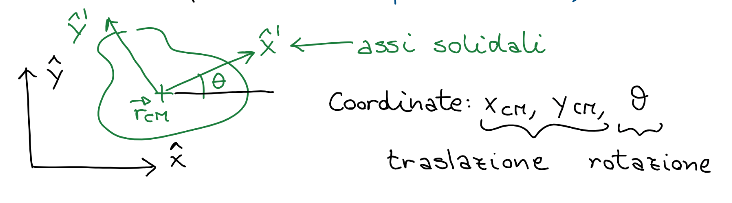
\includegraphics[width=0.65\textwidth]{images/geo-planare.png}
\end{figure}

\hspace{-15pt}Nella Geometria 3D (angoli di eulero):
\begin{figure}[h!]
    \centering
    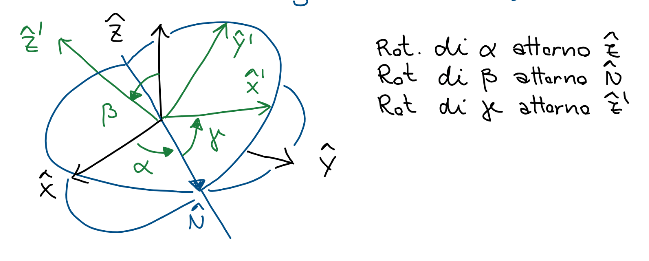
\includegraphics[width=0.55\textwidth]{images/geo-3d.png}
\end{figure}

\subsection{Teorema fondamentale sul moto del corpo rigido}
Il teorema fondamentale sul moto del corpo rigido dice che:
\begin{theorem}
    Ad ogni istante di tempo esiste ed è unico il vettore $\vec{w}(t)$, detto \textbf{vettore velocità angolare}, tale che, dati due punti qualunque $P_1, P_2$
    solidali al C.R.
    $$\dot{\vec{r}}_2(t) = \dot{\vec{r}}_1(t) + \vec{w}(t) \times [\vec{r}_2(t) - \vec{r}_1(t)]$$
    Dove $\vec{w}(t)$ è lo stesso per tutti i punti.
\end{theorem}
\hspace{-15pt}Sviluppiamo la teoria in modo generale, ma in questo corso incontriamo solo i moti planari dove:
$$\vec{r}_{\alpha}(t) = x(t) \hat{x} + y(t)\hat{y} + 0 \cdot \hat{z} \Rightarrow \vec{w}(t) = w(t) \hat{z}$$
\begin{example}
    $t= t_0, \vec{w}(t_0) = w\hat{z}, \dot{\vec{r}}_1(t_0) = v_0\hat{x}$
    $$\dot{\vec{r}}_2(t_0) = v_0\hat{x} + w\hat{z}x[L\hat{x}+ L\hat{y}] = v_0\hat{x} + wL\hat{y} - wL\hat{x} = (v_0 - wL)\hat{x} + wL\hat{y}$$
\end{example}
\begin{observation}
    Il vettore velocità angolare descrive il moto rotatorio del corpo rigido. Vogliamo quindi ottnere una equazione del moto per $\vec{w}(t)$ a partire dalla 2a Eq. 
    cardinale. Svolgiamo i passi necessari in questa lezione e nella prossima.
\end{observation}

\subsection{Momento angolare del corpo rigido}
Il momento angolare del corpo rigido si descrive come:
$$\vec{L}_p = M(\vec{r}_{CM}(t) - \vec{r}_p(t)) \times \dot{\vec{r}}_{CM}(t) + \sum_{\alpha=1}^{N}m_{\alpha}\vec{r}_{\alpha}'(t) \times \dot{\vec{r}}_{\alpha}'(t)$$
Con $M(\vec{r}_{CM}(t) - \vec{r}_p(t)) \times \dot{\vec{r}}_{CM}(t)$ dal CM. Mente $\vec{L}_{CM}(t) \equiv \sum_{\alpha=1}^{N}m_{\alpha}\vec{r}_{\alpha}'(t) \times \dot{\vec{r}}_{\alpha}'(t)$ rispetto al CM
\begin{equation*}
    \begin{split}
        \vec{L}_{CM}(t) & = \sum_{\alpha=1}^{N}[\vec{r}_{\alpha}(t) - \vec{r}_{CM}(t)] \times [\dot{\vec{r}}_{\alpha}(t) - \dot{\vec{r}}_{CM}(t)] = \sum_{\alpha=1}^{N} m_{\alpha}[\vec{r}_{\alpha}(t) - \vec{r}_{CM}(t)] \times [\vec{w}(t) \times [\vec{r}_{\alpha} - \vec{r}_{CM}(t)]]\\
                        & = \sum_{\alpha=1}^{N}m_{\alpha}[\vec{r}_{\alpha}'(t) \cdot \vec{r}_{\alpha}'(t)] \vec{w}(t) - \sum_{\alpha=1}^{N} m_{\alpha} \vec{r}_{\alpha}'(t)[\vec{r}_{\alpha}'(t) \cdot \vec{w}(t)]\\
                        & = \sum_{\alpha=1}^{N}m_{\alpha} 
                        \begin{pmatrix}
                            y_{\alpha}'^2 + z_{\alpha}'^2 & -x'_{\alpha} y'_{\alpha} & -x'_{\alpha}z'_{\alpha} \\
                            -y'_{\alpha}x'_{\alpha} & x_{\alpha}'^2 - z_{\alpha}'^2 & -y'_{\alpha}z'_{\alpha} \\
                            -z'_{\alpha}x'_{\alpha} & -z'_{\alpha}y'_{\alpha} & x_{\alpha}'^2 + y_{\alpha}'^2 
                        \end{pmatrix}
                        \begin{pmatrix}
                            w_{x'}(t)\\
                            w_{y'}(t)\\
                            w_{z'}(t)
                        \end{pmatrix}
    \end{split}
\end{equation*}
Coordinate nella base solidale: costante J.\\\\
La matrice J viene chiamata \textbf{tensore di inerzia} ed è una proprietà del corpo rigido, come la massa o il volume. $[J] = kg \cdot m^2$.
In 3D devo usare una matrice di rotazione con gli angoli di Eulero $w_{x'}, w_{y'}, w_{z'}$. Per moti planari (questo corso) $\vec{L}_p, \vec{L}_{CM}, \vec{w} // \hat{z}$
$$\vec{L}_{CM}(t) = \sum_{\alpha=1}^{N}m_{\alpha}(x_{\alpha}'^2 + y_{\alpha}'^2)w(t) \hat{z}$$
La parte $\sum_{\alpha=1}^{N}m_{\alpha}(x_{\alpha}'^2 + y_{\alpha}'^2)$ è detta $I_{CM}$ che sta per il momento di inerzia assiale. 
\begin{example}
    $I_{CM} = m_1|x_1'|^2 + m_2|x_2'|^2$ (ricordare che per la definizone $m_1x_1' + m_2x_2' = 0$)
\end{example}
\begin{example}
    Momento di inerzia assiale di un cilindro. $V= \pi R^2\cdot h \hspace{10pt}$ densità $\rho = M/V$
    $$I_z = \sum_{\alpha=1}^{N}m_{\alpha}(x_{\alpha}'^2 + y_{\alpha}'^2) = \int dm(x'^2 + y'^2) = \int dx' \int dy' \int_{0}^{h}dz' \cdot \rho(x'^2 + y'^2)$$
    Cambio di variabili nell'integrale per avere estremi più semplici: $x' = r \cdot \cos\Theta, y' = r \cdot \sin\Theta, dx' \cdot dy' = dr \cdot d\Theta \cdot r$
    $$= \int_{0}^{R}dr' \int_{0}^{2\pi}d\Theta' \cdot r'\int_{0}^{n}\cdot \rho \cdot r'^2 = \rho \cdot 2\pi \cdot h \cdot \frac{R^4}{4} = M\frac{1}{\pi R^2 h} \cdot 2\pi \cdot h \cdot \frac{R^4}{4} = \frac{1}{2}MR^2$$
    Posso calcolare il momento di inerzia assiale usando un punto solidale al C.R. diverso dal CM.
    \begin{equation*}
        \begin{split}
            I_p & = \sum_{\alpha=1}^{N}m_{\alpha}||\vec{r}_{\alpha} - \vec{r}_p(t)||^2 = \sum_{\alpha=1}^{N} m_{\alpha} ||\vec{r}_{\alpha}(t) - \underline{\vec{r}_{CM}(t) + \vec{r}_{CM}(t)} - \vec{r}_p(r)||^2\\
                & = \sum_{\alpha=1}^{N} m_{\alpha}\{||\vec{r}_{\alpha}(t) - \underline{\vec{r}_{CM}(t)}||^2 + ||\underline{\vec{r}_{CM}(t)} - \vec{r}_p(t)||^2 + 2[\vec{r}_{\alpha}(t) - \underline{\vec{r}_{\alpha}(t)}] \cdot [\underline{\vec{r}_{CM(t)} - \vec{r}_p(t)}]\}\\
                & = I_{CM} + M \cdot ||\underline{\vec{r}_{CM}(t)} - \vec{r}_p(t)||^2 + 2\underline{\{\sum_{\alpha=1}^{N}m_{\alpha}[\vec{r}_{\alpha}(t) - \vec{r}_{CM}(t)]\} \text{ (= 0) }} \cdot [\underline{\vec{r}_{CM}(t)} - \vec{r}_p(t)] \Rightarrow I_p = I_{CM} + M||\vec{r}_p||^2
        \end{split}
    \end{equation*}
    \underline{Teorema degli assi paralleli (Hyuhens - Steuiner)}
\end{example}

\begin{example}
    Cilindro con foto parallelo all'asse. Considero due cilindri fittizi di densità uguale al cilindro 1. Il 2 
    occupa lo spazio del foro, il 3 come 1 ma senza foto.
    $$            
    I_1^{(3)} = I_1^{(1)} + I_1^{(2)} \text{ (per additività del momento di interzia) } = I_1^{(1)} + I_1^{(2)} + M^{(2)} \cdot d^2\\
    $$
    \begin{equation*}
        \begin{split}
            I_1^{(1)} & = I_1^{(3)} - I_2^{2} - M^{(2)} d^2 = \frac{1}{2}(\rho v^{(3)})R^2 - \frac{1}{2}(\rho v^{(2)})R_2^2 - (\rho v^{(2)})d^2\\
                      & = \frac{1}{2}\rho h \pi((R^4) - R_2^4 - R_2^2 d^2) \:\:\:\:\underline{(g=\frac{M}{\pi R^2h})} \:\:\:\:= \frac{1}{2}MR^2[1 - \frac{R_2^4}{R^2} - \frac{R_2^2d^2}{R^4}] < \frac{1}{2}MR^2
        \end{split}
    \end{equation*} 
\end{example}
\hspace{-15pt}Equazioni cardinali per il corpo rigido:
$$
I. \:\: \ddot{M}\vec{r}_{CM}(t) = \sum_{i}\vec{F}_i(e)(t)
$$
Non importa il punto di applicazione delle forte \textbf{esterne} $\vec{F}_i^{(E)}(t)$
$$
II. \:\: \frac{d}{dt}[I_z\omega(t)\hat{z} + M[\vec{r}_{CM} - \vec{r}_p(t)] \times \dot{\vec{r}}_{CM}] = \sum_{i}[\vec{r}_i(t) - \vec{r}_p(t)] \times \vec{F}_i^{(E)}(t) - M\dot{\vec{r}}_p  \times \dot{\vec{r}}_{CM} 
$$
La parte $I_z\omega(t)\hat{z}$ è una forma semplificata valida solo per il modo nel piano $\hat{x}, \hat{y}$. Essenziale il punto di applicazione delle forze.
Polo $\vec{r}_p$ arbitrario, scelgo quello che semplifica.

\begin{example}
    Cilindro vincolato e forza costante. \\
    Scelto come polo il CM. $\vec{F} = - F\hat{x} \:\:\: \vec{N}= N \hat{x} \:\:\: \vec{\omega} = \dot{\Theta}\hat{z}$.\\
    Abbiamo che $N = F$ e nessuna info su $\Theta$. I vincoli sono: $\vec{r}_{CM}(t) \equiv 0 \Rightarrow \ddot{\vec{r}}_{CM}(t) = 0$
    \begin{itemize}
        \item $I. \:\: M\ddot{\vec{r}}_{CM} = \vec{F} + \vec{N} = (N - F)\hat{x}$
        \item $II. \:\: \frac{d}{dt}[I_z\omega(t)\hat{z} + M[\vec{r}_{CM}(t) - \vec{r}_p(t)] \times \dot{\vec{r}}_{CM}] = \sum_{i}[\vec{r}_i(t) - \vec{r}_p(t)] \times \vec{F}_i^(E)(t) - M\dot{\vec{r}}_p \times \dot{\vec{r}}_{CM}$
    \end{itemize}
    $$I_z\dot{\omega}(r)\hat{z} = (\vec{r}_i - \vec{r}_{CM}) \times \vec{F} + (\vec{r}_{CM} - \vec{r}_{CM}) \times \vec{N} = R\hat{y} \times (-F\hat{x}) + 0 = RF\hat{z} \Rightarrow I_z\ddot{\Theta}(t) = RF \hspace{10pt}\ddot{\Theta} = \frac{2F}{MR} \text{ costante}$$
\end{example}

\subsection{Condizione del "puro rotolamento"}
Il punto $\vec{r}_1$ del corpo rigido a contatto con la superficie al tempo $t_1$ è fermo. Al tempo 
$t_2$ un altro punto $\vec{r}_2$ del corpo rigido è a contatto con la superfice. Il punto geometrico $\vec{r}_C(t)$ di contatto 
\textbf{non è solidale} e il suo moto non è determinato dal vettore $\vec{w}(t)$
\begin{figure}[h!]
    \centering
    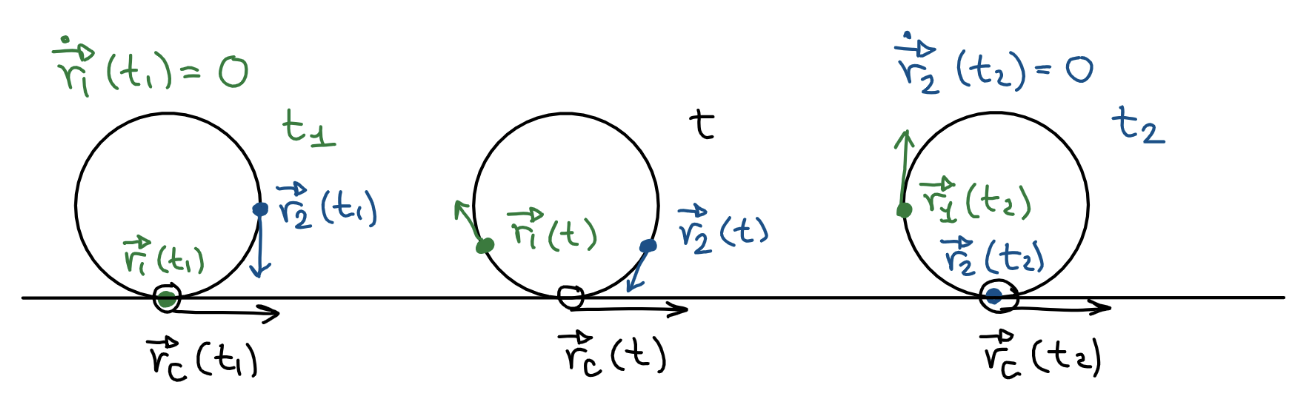
\includegraphics[width=0.65\textwidth]{images/puro-rotolamento.png}
\end{figure}
\begin{example}
    Cilindro trainato su piano scabro.
    \begin{figure}[h!]
        \centering
        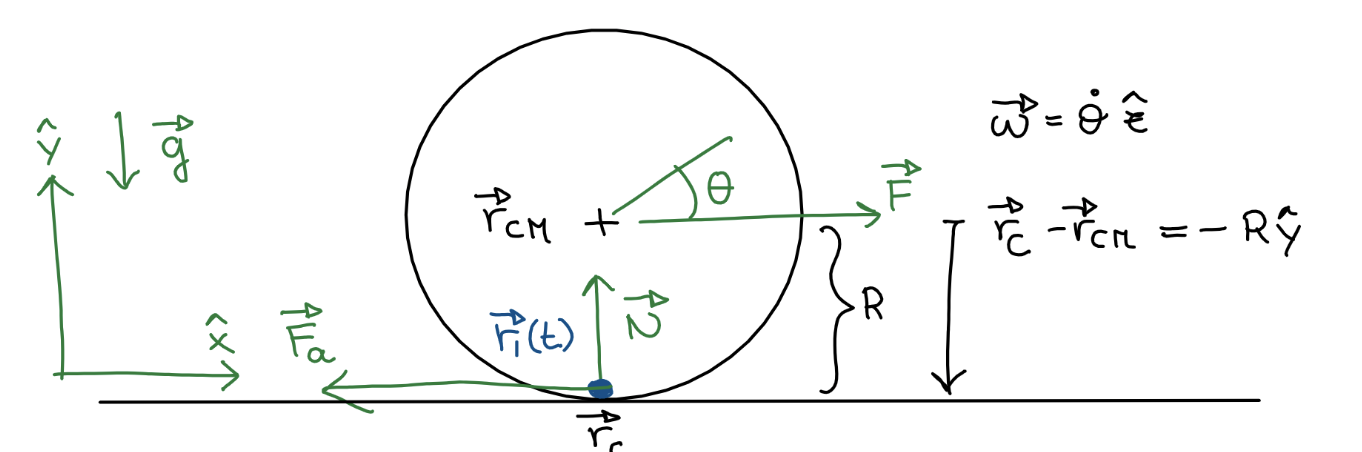
\includegraphics[width=0.50\textwidth]{images/cilindro-trainato-piano-scabro.png}
    \end{figure}
    \begin{itemize}
        \item $I. \:\: O = M\ddot{y}_{CM}(t) = -Mg + N \Rightarrow N = mg \hspace{15pt} M\underline{\ddot{x}_{CM}} = F - F_a$
        \item $II. \:\: I_z\underline{\dot{\omega}(t)}\hat{z} = (\vec{r}_{CM} - \vec{r}_{CM}) \times \vec{F} + (\vec{r}_{CM} - \vec{r}_CM) \times (\vec{F}_a + \vec{N}) = 0 + (-R\hat{y}) \times (-F_a\hat{x} + N\hat{y}) = -RF_a\hat{z}$
    \end{itemize}
    \underline{Abbiamo 3 incognite}.
\end{example}
\hspace{-15pt}Vincolo del puro rotolamento
$$0 = \dot{\vec{r}}_{CM}(t) + \vec{\omega} \times [\vec{r}_c(t) - \vec{r}_{CM}(t)]$$
Ma quando il punto $\vec{r}_1$ è a contatto $\vec{r}_1(t) = \vec{r}_C(t) \Rightarrow 0 = \dot{\vec{r}}_{CM}(t) + \vec{\omega} \times [\vec{r}_C(t) - \vec{r}_{CM}(t)]$ 
$$ = \dot{x}_{CM}(t)\hat{x} + \dot{\Theta}(t)\hat{z} \times (-R\hat{y}) = \dot{x}_{CM}(t)\hat{x} + R \dot{\Theta}(t)\hat{x} \Rightarrow \underline{\dot{x}_{CM}(t) = -R\dot{\Theta}(t)} \Rightarrow \ddot{x}_{CM}(t) = -R\ddot{\Theta}(t)$$
Sostituisco nelle equazioni cardinali
$$
\begin{cases}
    -MR\ddot{\Theta} = F - F_a\\
    \frac{1}{2}MR^2 \ddot{\Theta} = -RF_a
\end{cases}
\:\:\:
\begin{cases}
    F_a = -\frac{1}{2}MR\ddot{\Theta}\\
    -MR\ddot{\Theta} = F + \frac{1}{2}MR\ddot{\Theta}
\end{cases}
\begin{cases}
    \ddot{\Theta} = -\frac{2}{3}\frac{F}{MR}\\
    F_a = \frac{1}{3}F
\end{cases}
$$
Minimo $\mu_s$ per mantenere puro rotolamento?
$|F_a| \leq \mu_S|N| \hspace{15pt} \mu_S \geq \frac{F/3}{Mg} = \mu_s,min$

\subsection{Energia del corpo rigido}
$$K(t) = \frac{1}{2}M||\dot{\vec{r}}_{CM}(t)||^2 + \sum_{\alpha=1}^{N}\frac{1}{2}m_{\alpha}||\dot{\vec{r}}_{\alpha}'(t)||^2$$
Con $\frac{1}{2}M||\dot{\vec{r}}_{CM}(t)||^2$ dal CM e $\sum_{\alpha=1}^{N}\frac{1}{2}m_{\alpha}||\dot{\vec{r}}_{\alpha}'(t)||^2$ rispetto al CM $\equiv K_{CM}(t)$
	\newpage
\section{Urto}
Un \textbf{urto} tra punti materiali / corpi rigidi avviene in un intervallo temporale 
$t_0 - \epsilon < t < t_0 + \epsilon$ molto breve, rispetto alla dinamica del sistema.\\\\
Le reazioni vincolari sono difficili da descrivere con precisione. Ci interessa invece lo stato del sistema \textbf{subito prima}
($t_0^- \equiv t_0 - \epsilon$) e \textbf{subito dopo} ($t_0^+ = t_0 \epsilon$). 
Durante l'urto le forze che non sono generate dal contatto sono spesso di intensità trascurabile.
\begin{definition}
    Definisco \textbf{vetore impulso di una forza} $\vec{F}(t)$ un intervallo temporale $[t_0 - \epsilon, t_0 + \epsilon]$
    $$\vec{I}_{\epsilon} = \int_{t_0 - \epsilon}^{t_0 + \epsilon}dt \cdot \vec{F}(t) \hspace{10pt} \text{e} \hspace{10pt}\vec{I} = \lim_{\epsilon\to 0}\vec{I}_{\epsilon}$$
\end{definition}
Dico che $\vec{F}(t)$ è una \textbf{forza impulsiva} se $||\vec{I}|| \neq 0$ altrimenti la forza è non impulsiva.
Una forza la cui intensità è limitata non può essere impuliva.\\\\
Le coordinate sono funzioni continue del tempo (non ci può essere "teletrasposrto"), ess. $\vec{r}(t_0^+) = \vec{r}(t_0^-)$ mentre
velocità, accelerazione, quantità di moto, momento angolare, energia cinetica possono subire variazioni tra $t_0 - \epsilon$ e $t_0 + \epsilon$.\\\\
Se l'energia cincetica \textbf{del sistema} non vaira tra $t_0 - \epsilon$ e $t_0 + \epsilon$ ("è conservata") l'urto si dice \textbf{elastico}, altrimenti \textbf{anelastico}.
Se dopo l'urto si viene a formare un corpo rigido, l'urto è \textbf{completamente anelastico}.

\subsection{Equazioni cardinali e teorema forze vive in forma impulsiva}
Integro entrabi i membri da $t_0 - \epsilon$ a $t_0 + \epsilon$
$$I. \:\:\: m\ddot{\vec{r}}_{CM}(t) = \sum_i \vec{F}_i^{(E)}(t) \Rightarrow m\dot{\vec{r}}_{CM}(t_0^+) - m\dot{\vec{r}}_{CM}(t_0^-) = \sum_i \vec{I}_i^{(E)}$$
$\vec{I}_i^{(E)}$ vuol dire che sono le $\vec{F}_i$ impulsive contano.
$$II. \:\:\: \dot{\vec{L}}_p(t) = \sum_i(\vec{r}_i(t) - \vec{r}_p(t)) \times \vec{F}_i^{(E)} - \dot{\vec{r}}_p(t) \times M\dot{\vec{r}}_{CM}(t) \Rightarrow \vec{L}_p(t_0^+) - \vec{L}_p(t_0^-) = \sum_i(\vec{r}_i(t_0) - \vec{r}_p(t_0)) \times \vec{I}_i(E)$$
Anche in questo caso sole le $\vec{F}_i$ impulsive contano, in oltre come si nota in $M\dot{\vec{r}}_{CM}(t)$ le velocità rimangono limitate.
\begin{example}
    Non ci sono forze esterne impulsive.
    $$m_i\dot{x}_i(t_0^+) + m_2\dot{x}_2(t_0^+) - m_1\dot{x}_1(t_0^-) - m_2\dot{x}_2(t_0^-) = 0$$
    ($\dot{x}_1(t_0^-) = v_1$ e $ m_2\dot{x}_2(t_0^-) = v_2$) \hspace{5pt}L'urto è elastico
    $$\frac{1}{2}m_1\dot{x}_1(t_0^+)^2 + \frac{1}{2}m_2\dot{x}_2(t_0^+)^2 - \frac{1}{2}m_1\dot{x}_1(t_0^-)^2 - \frac{1}{2}m_2\dot{x}_2(t_0^-)^2 = 0$$
    $$\Rightarrow \dot{x}_2 (t_0^+) = v_2 - \frac{m_1}{m_2}[\dot{x}_1 (t_0^+) - v_1] \Rightarrow \frac{1}{2}m_1\dot{x_1}(t_0^+)^2 + \frac{1}{2}m_2 \{v_2 - \frac{m_1}{m_2}[\dot{x_1}(t_0^+) - v_1]\}^2$$
    $$-\frac{1}{2}m_1 v_1^2 - \frac{1}{2}m_2v_2^2 = 0$$
    $$\dot{x}_1(t_0^+) = \frac{m_1 - m_2}{m_1 + m_2}v_1 + \frac{2m_2}{m_1+m_2}v_2$$
\end{example}
\begin{example}
    Piano liscio, urto elastico. Liscio: la relazione vincolare impulsiva è solo normale.
    $$\begin{cases}
        m\dot{x}(t_0^+) - m\dot{x}(t_0^-) = 0\\
        m\dot{y}(t_0^+) - m\dot{y}(t_0^-) = N \text{ impulso relazione vincolare}
    \end{cases}$$
    $$\frac{1}{2}m[\dot{x}(t_0^+)^2 + \dot{y}(t_0^+)^2] - \frac{1}{2}m[\dot{x}(t_0^-)^2 + \dot{y}(t_0^-)^2] = 0 \Rightarrow \dot{x}(t_0^+) = \dot{x}(t_0^-) \text{ non cambia }$$
    $$\dot{y}(t_0^+)^2 - \dot{y}(t_0^-)^2 = 0 \Rightarrow \dot{y}(t_0^+) - \dot{y}(t_0^-) \text{ si inverte } \Rightarrow N = 2m\dot{y}(t_0^-)$$
\end{example}
\begin{example}
    Minimo $\mu_s$ per un "wallrun"?
    $$\dot{\vec{r}}(t_0^-) = v_1 \hat{x} \hspace{15pt} \dot{\vec{r}}(t_0^+) = v_2\hat{y}$$
    $$
    \begin{cases}
        m\dot{x}(t_0^+) - m\dot{x}(t_0^-) = -N\\
        m\dot{y}(t_0^+) - m\dot{y}(t_0^-) = I_a
    \end{cases}
    \Rightarrow
    \begin{cases}
        N = mv_1 \\
        I_a = mv_2
    \end{cases}
    $$
    Da $||\vec{F}_a|| \leq \mu_s||\vec{N}||$, integrando membro a membro, segue $I_a \leq \mu_s N \Rightarrow \mu_s \geq \frac{mv_2}{mv_1} = \frac{v_2}{v_1} = \mu_s,min$
\end{example}
\begin{example}
    Urto anelastico asta-perno. Massimo $\Theta$?\\
    L'urto forza esterna impulsiva è la relazione vincolare in P, che però ha momento nullo rispetto a P.
    $$\vec{L}_p(t_0^+) - \vec{L}_p(t_0^-) = 0 \hspace{10pt}\vec{L}_p(t_0^-) = (\vec{r}_{CM}(t_0^-) - \vec{r}_p) \times M\dot{\vec{r}}_{CM}(t_0^-) = -\frac{L}{2}\hat{y} \times Mv_0 \hat{x} = \frac{1}{2}MLv_0\hat{z}$$
    Solo il momento angolare "del CM" è non nullo.
    $$\vec{L}_p(t_0^+) = \frac{1}{2}ML \frac{L}{2}\dot{\Theta}(t_0^+)\hat{z} + (\frac{1}{12}ML^2)\dot{\Theta}(t_0^+)\hat{z} = \frac{1}{3}ML^2 \dot{\Theta}(t_0^+)\hat{z}$$
    $$\frac{1}{3}ML^2\dot{\Theta}(t_0^+) - \frac{1}{2}MLv_0 = 0 \Rightarrow \dot{\Theta}(t_0^+) = \frac{3}{2}\frac{v_0}{L}$$
    Per $t > t_0$ l'energia si conserva perché le forze che fanno lavoro sono conservative. La relazione in P non è conservativa ma P è fermo e c'è attrito.
    $$\frac{1}{2}M[\frac{L}{2}\dot{\Theta}(t_0^+)]^2 + \frac{1}{2}(\frac{1}{12}ML^2)\dot{\Theta}(t_0^+)^2 - Mg\frac{L}{2} = -Mg \frac{L}{2}\cos\Theta_{max}$$
    $$\Rightarrow Mg \frac{L}{2}(1 - \cos\Theta_{max}) = \frac{1}{1}\cdot \frac{1}{3}ML^2\dot{\Theta}(t_0^+)^2 = \frac{1}{6}ML^2 \frac{g}{4} - \frac{v_0^2}{L^2} \Rightarrow 1 - \cos\Theta_{max} = \frac{3}{4}\frac{v_0^2}{gL} \hspace{10pt}\Theta_{max} = \arccos(1-\frac{3}{4}\frac{v_0^2}{gL})$$
\end{example}
\end{document}
